%%%%%%%%%%%%%%%%%%%%%%%%%%%%%%%%%%%%%%%%%%%%%%%%%%%%%%%%%%%%%%%%%%%%%%%%%%%%%%
%
% MASTER FILE START
%
%%%%%%%%%%%%%%%%%%%%%%%%%%%%%%%%%%%%%%%%%%%%%%%%%%%%%%%%%%%%%%%%%%%%%%%%%%%%%%

\documentclass{beamer}
\usepackage{etex}
\mode<presentation> {
\usetheme{Singapore}
\setbeamercovered{invisible}
\setbeamertemplate{navigation symbols}{} 
}
%%%%%%%%%%%%%%%%%%%%%%%%%%%%%%%%%%%%%%%%%%%%%%%%%%%%%%%%%%%%%%%%%%%%%%%%%%%%%%
%
% PACKAGES
%
%%%%%%%%%%%%%%%%%%%%%%%%%%%%%%%%%%%%%%%%%%%%%%%%%%%%%%%%%%%%%%%%%%%%%%%%%%%%%%
\usepackage[absolute,overlay]{textpos}
\newcommand{\tikzmark}[1]{\tikz[overlay,remember picture] \node (#1) {};}
\graphicspath{{./figures/}}
\usepackage{cancel}
\usepackage{url}               % url typeset correctly
\usepackage{named}
\usepackage{tikz}
\usepackage{picture}
\usepackage{algorithm,algorithmic}
\usepackage{multirow}
\usepackage{proof}
\usepackage{transparent}
\usepackage{url}
\usepackage{hyperref}	
\newcommand*\rot{\rotatebox{60}}
\usepackage{color, colortbl}
\usepackage[first=0,last=9]{lcg}
\newcommand{\ra}{\rand0.\arabic{rand}}
\newcommand\FrameText[1]{%
  \begin{textblock*}{\paperwidth}(261pt,239pt)
    \raggedright #1\hspace{.5em}
  \end{textblock*}}

\definecolor{LightCyan}{rgb}{1,0.88,1}

\setlength{\inferLineSkip}{4pt}
%\usepackage[inference]{semantic}
\usetikzlibrary{shapes,arrows,snakes,backgrounds,%
matrix,patterns,arrows,decorations.pathmorphing,decorations.pathreplacing,%
positioning,fit,calc,decorations.text, automata%
}
\newcommand{\hilightgray}[1]{\colorbox{gray!38}{#1}}
\newcommand{\hilightgreen}[1]{\colorbox{darkgreen!38}{#1}}

\definecolor{gray}{rgb}{0.4,0.4,0.4}
\definecolor{darkblue}{rgb}{0.0,0.0,0.6}
\definecolor{darkbl}{rgb}{0.0,0.0,0.6}
\definecolor{cyan}{rgb}{0.0,0.6,0.6}
\definecolor{darkgreen}{rgb}{0,0.46,0}
\def\checkmark{\tikz\fill[scale=0.4](0,.35) -- (.25,0) -- (1,.7) -- (.25,.15) -- cycle;} 
\setbeamertemplate{blocks}[rounded][shadow=false]
\newlength{\Size}

%%% Grid on the slides

% \usepackage[texcoord,grid,gridunit=mm,gridcolor=red!10,subgridcolor=green!10]
% {eso-pic}

\usepackage{enumerate}
\usepackage{amstext}
\usepackage{amssymb}
\usepackage{amsbsy}
\usepackage{amsmath}
\usepackage{color}
\usepackage[absolute,overlay]{textpos}
\usepackage{cancel}

\mode<article>
{
\usepackage{fullpage}
}

\def\uminus{\setbox0=\hbox{$\cup$}\rlap{\hbox
    to\wd0{\hss\raise0.3ex\hbox{$\scriptscriptstyle{-}$}\hss}}\box0}
\def\cminus{\setbox0=\hbox{$\cap$}\rlap{\hbox
    to\wd0{\hss\raise0.3ex\hbox{$\scriptscriptstyle{-}$}\hss}}\box0}
\definecolor{light-gray}{gray}{0.45}

\usepackage{soul}




%%%%%%%%%%%%%%%%%%%%%%%%%%%%%%%%%%%%%%%%%%%%%%%%%%%%%%%%%%%%%%%%%%%%%%%%%%%%%%
%
% CUSTOM BEAMER STYLE
%
%%%%%%%%%%%%%%%%%%%%%%%%%%%%%%%%%%%%%%%%%%%%%%%%%%%%%%%%%%%%%%%%%%%%%%%%%%%%%
\setbeamertemplate{blocks}[rounded][shadow=false]
% setup margin
\beamersetleftmargin{0.5cm}
\beamersetrightmargin{0.5cm}

% setup symbols
\setbeamertemplate{bibliography item}[book]
\setbeamertemplate{navigation symbols}{} % turn off navigation symbols

% setup font shapes of various elements
\setbeamerfont{frametitle}{series=\bfseries}
%\setbeamercolor{alerted text}{series=\bfseries}

% put number of frames at the bottom
\setbeamertemplate{footline}[frame number]


\usepackage[scaled]{helvet}

\newtheorem{proposition}[theorem]{Proposition}


\setbeamercolor{alerted text}{fg=purple}

\newcommand{\makeoverview}{%
  \begin{frame}
    \frametitle{Outline}
    \tableofcontents
  \end{frame}
}

\newcommand{\makereferences}[1]{%
  \begin{frame}[allowframebreaks,allowdisplaybreaks]
    \frametitle{References}
    \bibliography{#1}
  \end{frame}
}



%%%%%%%%%%%%%% SPACING COMMANDS 

\newcommand{\bs}{\bigskip}
\newcommand{\m}{\medskip}
\newcommand{\s}{\smallskip}


%%%%%%%%%%%%%% SPECIFIC MACROS
\newcommand{\weak}{\ensuremath{\mathit{weak}}}
\newcommand{\FLP}{\ensuremath{\mathit{flp}}}
\newcommand{\wred}[3]{\ensuremath{{#1^{#2,#3}_{\mi{weak}}}}}
\newcommand{\flpred}[3]{\ensuremath{{#1^{#2,#3}_{\mi{flp}}}}}
\newcommand{\citeY}[1]{\citeyear{#1}}
\newcommand{\naf}{{\it not}\,}
\newcommand{\NP}{\ensuremath{\mathrm{NP}}}
\newcommand{\SigmaP}[1]{{\Sigma}_{#1}^{P}}
\newcommand{\wrt}[0]{w.r.t.\ }
\newcommand{\tuple}[1]{\ensuremath{\langle#1\rangle}}
\renewcommand{\vec}[1]{\ensuremath{\mathbf{#1}}}
\newcommand{\dlliteplugin}{{\fontencoding{OT1}\fontfamily{cmss}\selectfont{dlliteplugin}}}
\newcommand{\hnbls}{\vspace*{-.5\baselineskip}}
\newcommand{\bl}[1]{\textcolor{blue}{#1}}
\newcommand{\gr}[1]{\textcolor{darkgreen}{#1}}
\usepackage{mathtools}
\newcommand{\prg}{\mathcal{P}}
\newcommand{\gre}[1]{\textcolor{darkgreen}{#1}}
\newcommand{\dllite}{\ensuremath{DL}\text{-}\ensuremath{Lite}}
\newcommand{\el}{\ensuremath{\mathcal{EL}}}
\newcommand{\specialcell}[2][l]{\begin{tabular}[#1]{@{}c@{}}#2\end{tabular}}
   \newcommand*\circled[1]{%
      \tikz[baseline=(C.base)]\node[draw,circle,inner sep=1pt](C) {#1};\!
    }
   \newcommand*\circledbl[1]{%
      \tikz[baseline=(C.base)]\node[draw,circle,fill=blue!10,inner sep=1.7pt](C) {#1};\!
    }

\usepackage{color}
\newcommand{\hilightbl}[1]{\colorbox{darkblue!18}{#1}}
\newcommand{\hilightred}[1]{\colorbox{red!18}{#1}}

\setbeamercolor{uppercolblue}{fg=black,bg=darkbl!25}
\setbeamercolor{lowercolblue}{fg=black,bg=darkbl!0}

\setbeamercolor{uppercolgreen}{fg=black,bg=darkgreen!35}
\setbeamercolor{lowercolgreen}{fg=black,bg=darkgreen!12}

\setbeamercolor{uppercolred}{fg=black,bg=red!30}
\setbeamercolor{lowercolred}{fg=black,bg=red!12}

\def\cA{\ensuremath{\mathcal{A}}}
\def\cG{\ensuremath{\mathcal{G}}}
\def\cT{\ensuremath{\mathcal{T}}}
\def\cI{\ensuremath{\mathcal{I}}}
\def\cC{\ensuremath{\mathcal{C}}}
\def\cO{\ensuremath{\mathcal{O}}}
\def\cR{\ensuremath{\mathcal{R}}}
\def\cP{\ensuremath{\mathcal{P}}}
\newcommand{\dlvhex}{\textsf{dlvhex}}
\usepackage{appendixnumberbeamer}

\definecolor{darkblue}{rgb}{0.0, 0.62,0.9}

\newcommand\hex{{\sc hex}}

\catcode`\@=11 % as in plain.tex
\long\def\blank#1{\bl@nk#1@@..\bl@nk}%
\long\def\bl@nk#1#2@#3#4\bl@nk{#3#4}
\catcode`\@=12

\long\def\test#1{\begingroup \toks0{[#1]}%
  \newlinechar`\/\message{/\the\toks0:
  \if\blank{#1}EMPTY\else NOT empty\fi%
}\endgroup}



\newcommand{\mi}[1]{\ensuremath{\mathit{#1}}}
\newcommand{\mb}[1]{\ensuremath{\mathbf{#1}}}
\newcommand{\tbf}[1]{\textbf{#1}}
\newcommand{\dlatom}[3]{\ensuremath{{\operatorname{DL}}{[#1;#2]}{(#3)}}}


%%%%%%%%%%%%%%%%%%%%%%%%%%%%%%%%%%%%%%%%%%%%%%%%%%%%%%%%%%%%%%%%%%%%%%%%%%%%%%
%
% DOCUMENT PROPERTIES
%
%%%%%%%%%%%%%%%%%%%%%%%%%%%%%%%%%%%%%%%%%%%%%%%%%%%%%%%%%%%%%%%%%%%%%%%%%%%%%%


\title{Towards Nonmonotonic Relational Learning from Knowledge Graphs}
 \author[Stepanova]
 {
   \large{}\\
 }

\author[shortname]{\underline{Hai Dang Tran\inst{1}}, Daria Stepanova\inst{1}, Mohamed Gad Elrab\inst{1},\\ Francesca A. Lisi\inst{2}, Gerhard Weikum\inst{1}
}
\institute[shortinst]{\inst{1} Max Planck Institute for Informatics, Saarbr\"{u}cken, Germany \and %
                      \inst{2} Universit\`{a} degli Studi di Bari ``Aldo Moro", Bari, Italy}



  \bigskip
\titlegraphic{
  \centering

 
\includegraphics[height=1cm]{logo_mpi_430} \\\includegraphics[height=2.3cm]{logo_bari}

 \large{}
}
 \date[]{}

%%%%%%%%%%%%%%%%%%%%%%%%%%%%%%%%%%%%%%%%%%%%%%%%%%%%%%%%%%%%%%%%%%%%%%%%%%%%%%
%
% DOCUMENT START
%
%%%%%%%%%%%%%%%%%%%%%%%%%%%%%%%%%%%%%%%%%%%%%%%%%%%%%%%%%%%%%%%%%%%%%%%%%%%%%%

\begin{document}

\frame{\titlepage}
\addtocounter{framenumber}{-1}


%%%%%%%%%%%%%%%%%%%%%%%%%%%%%%%%%%%%%%%%%%%%%%%%%%%%%%%%%%%%%%%%%%%%%%%%%%%%%%
\section{Introduction}
\begin{frame}\frametitle{Introduction}
\medskip
\begin{itemize}
\small{\item \textcolor{blue}{Knowledge Graphs}: a large collection of facts $\tuple{subject\;predicate\;object}$
\begin{itemize}
\item[] \gr{$\tuple{\mi{Brad\;isMarriedTo\;Ann}}$, $\tuple{\mi{Dave \;type\;Researcher}}$}
\end{itemize}
\bigskip

\item Represent unary/binary facts with \textcolor{blue}{Open World Assumption (OWA)}
\begin{itemize}
\item[] \gr{$\mi{isMarriedTo(Brad,Ann), Researcher(Dave)}$}
\end{itemize}
\bigskip

\item KGs are normally \bl{incomplete} and contains \bl{inaccurate} facts
}
\end{itemize}

\begin{figure}[ht]
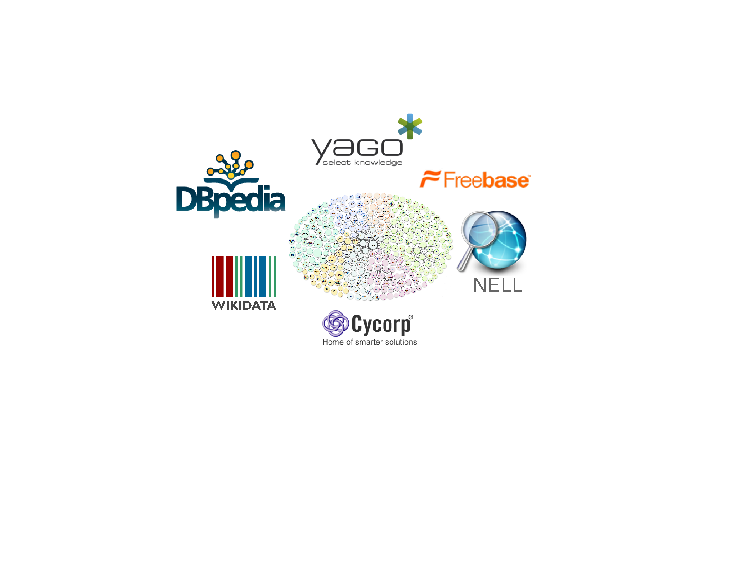
\includegraphics[width=0.5\textwidth]{kb}
\caption{Typical Knowledge Graphs~\cite{rumis}.}
\end{figure}

%\begin{picture}(0.5,0.5)
%\put(60,-110){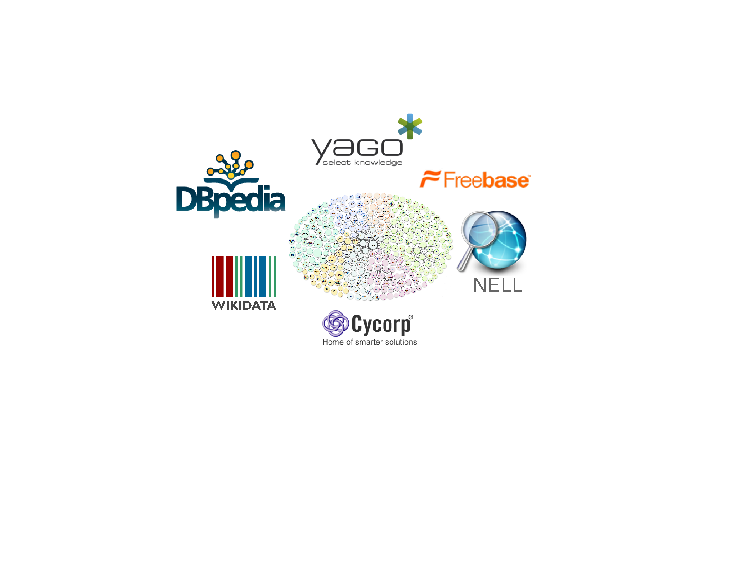
\includegraphics[width=0.65\textwidth]{kb}}
%\caption{abc}
%\end{picture}

\end{frame}

\begin{frame}\frametitle{Introduction}
\alt<3->{\bl{In this thesis:} relational nonmonotonic rule mining under \alert{OWA}}{\bl{Complete} KGs with \bl{positive rule} mining \cite{amie}}
 \bigskip
 \bigskip
 \bigskip
 \bigskip
 \bigskip
 \bigskip
 \bigskip
 \bigskip
 \bigskip
 \bigskip
 \bigskip
 \bigskip
 \bigskip
 \bigskip
 \bigskip
 \bigskip
 \bigskip
 \bigskip

\alt<3->{
\begin{picture}(0.5,0.5)\put(43,-43){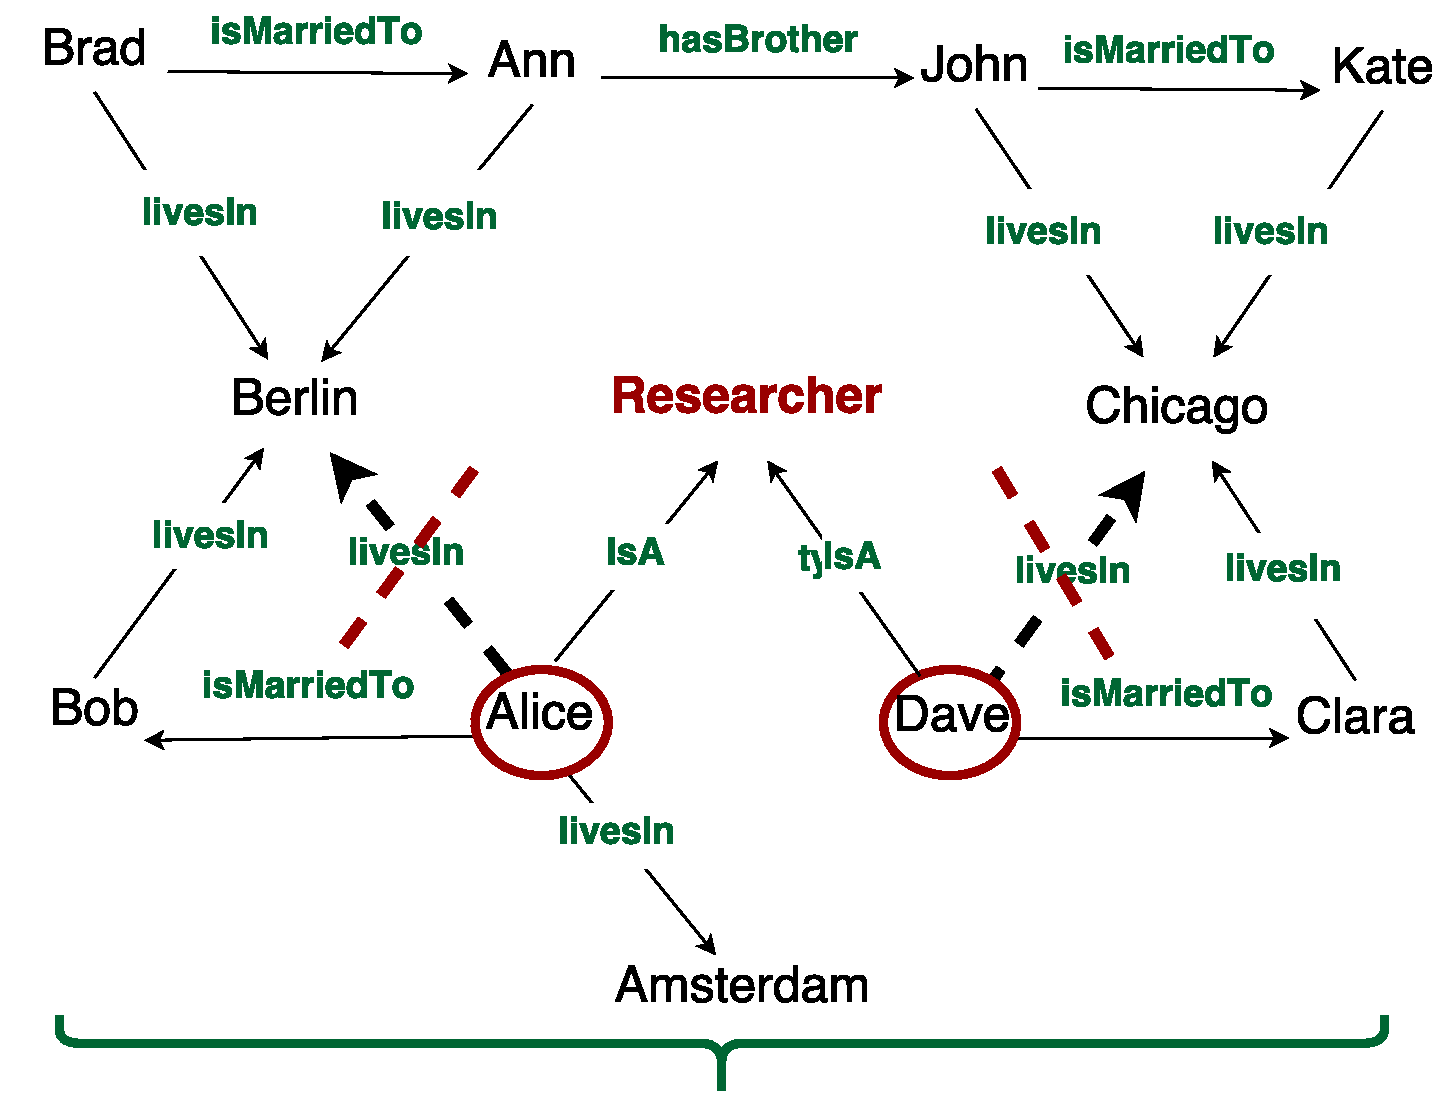
\includegraphics[width=0.75\textwidth]{kg_2}}\end{picture}
}{\alt<2->{\begin{picture}(0.5,0.5)\put(43,-43){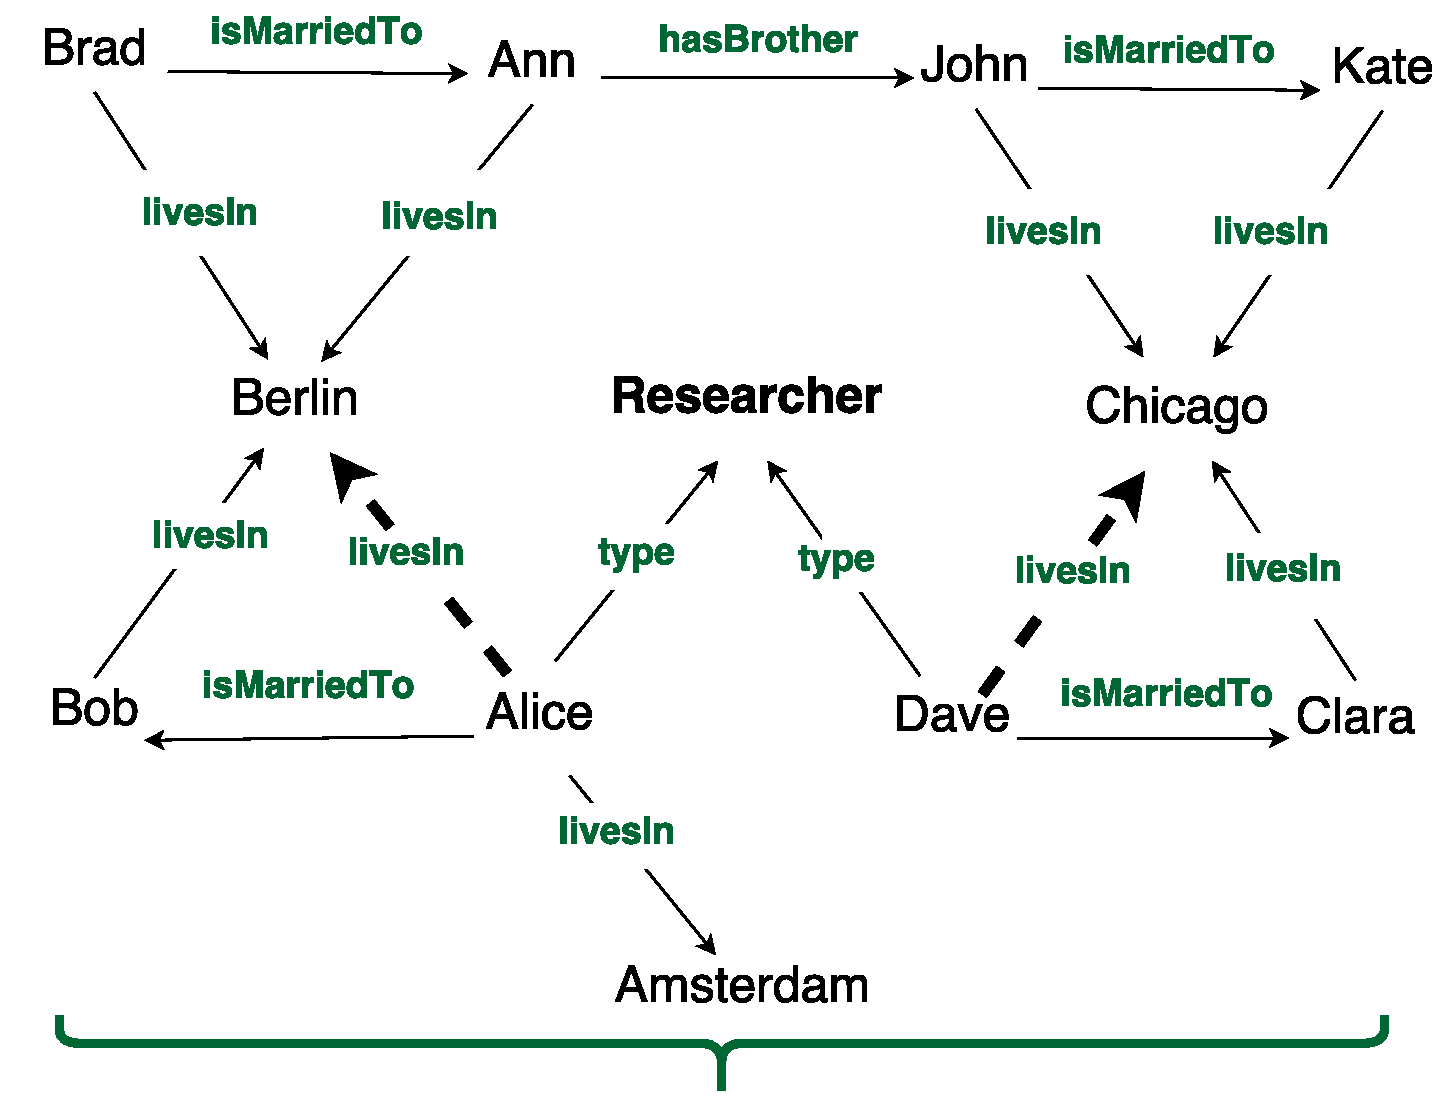
\includegraphics[width=0.75\textwidth]{kg_1_5}}\end{picture}}{\begin{picture}(0.5,0.5)\put(43,-42){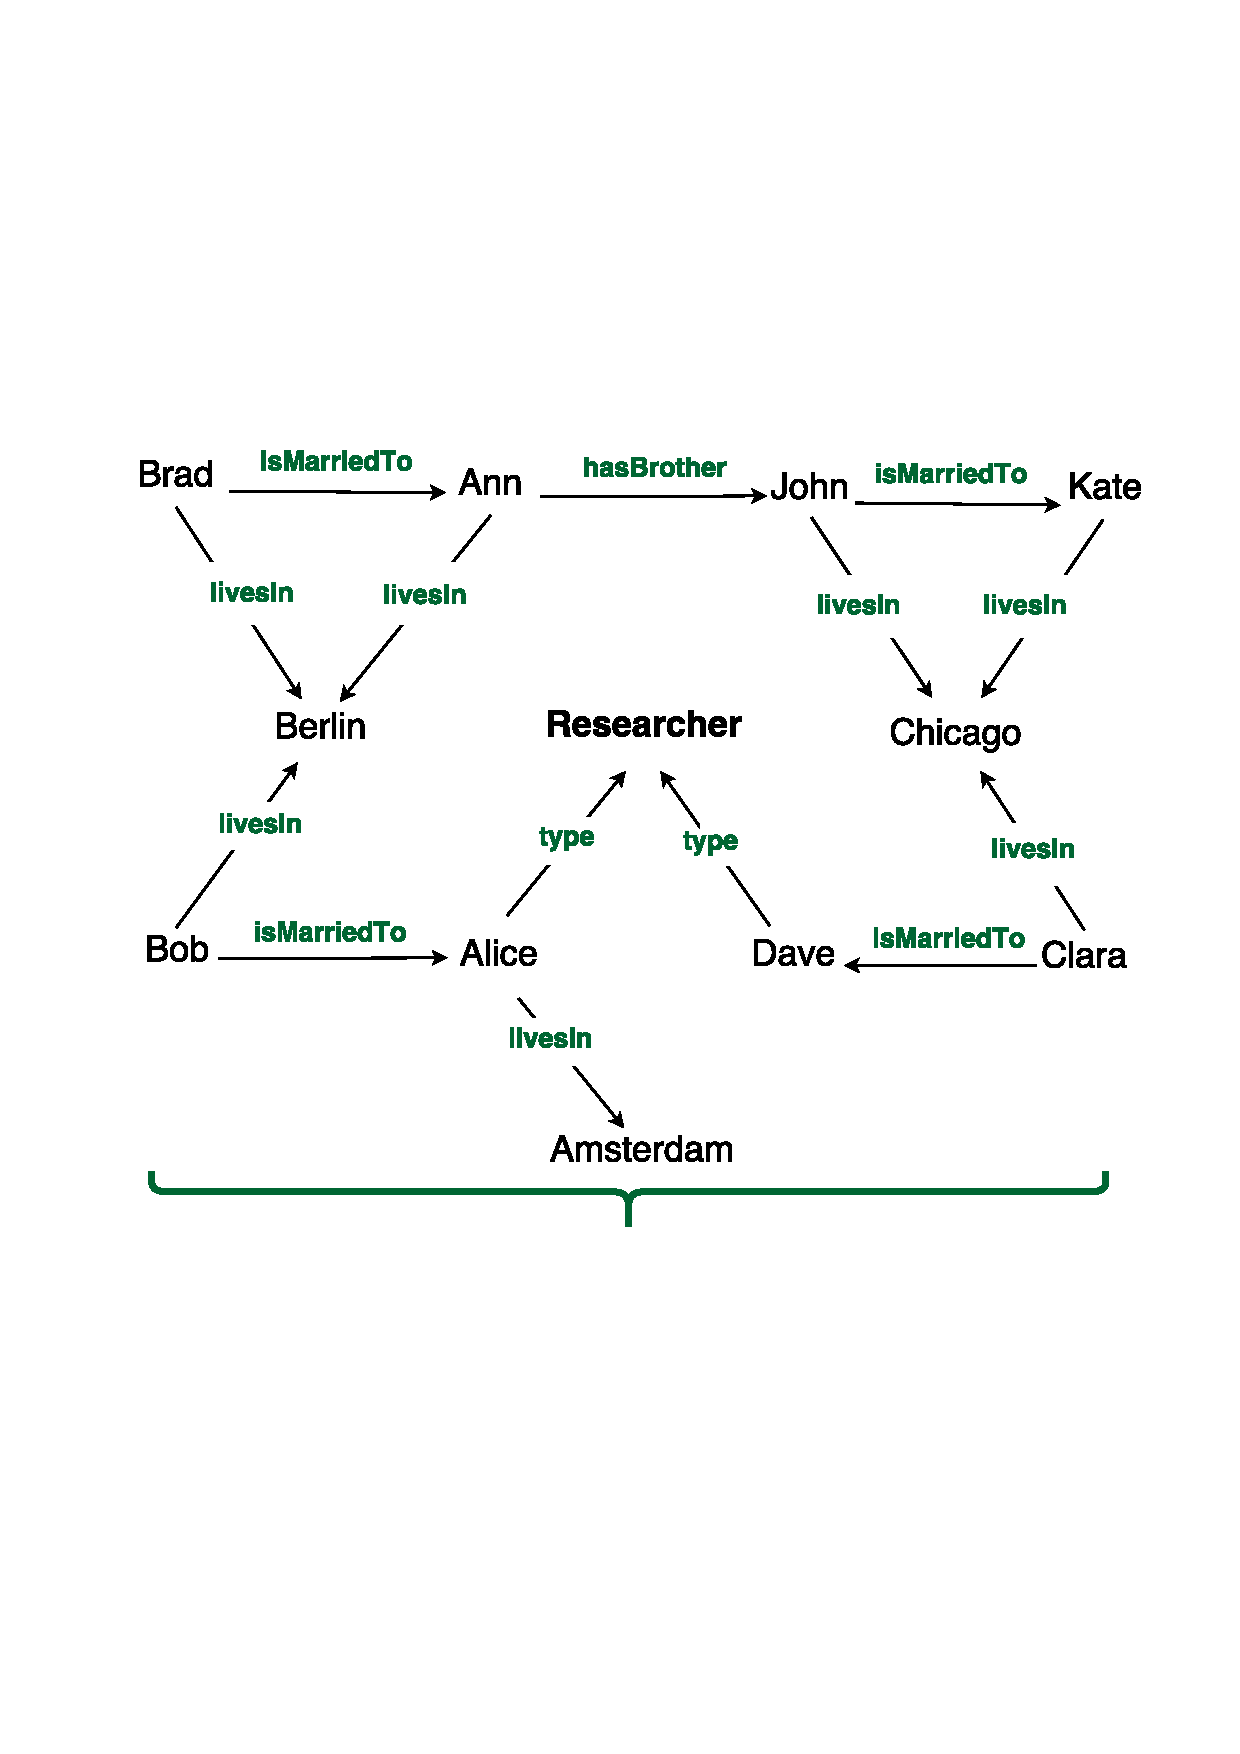
\includegraphics[width=0.75\textwidth]{kg_1}}\end{picture}}}
\begin{center}
\bigskip
\bigskip
\bigskip
\bigskip

\normalsize{\alt<3>{\textcolor{darkgreen}{$r:\;\mi{livesIn(X,Z)}\leftarrow \mi{isMarriedTo(X,Y),livesIn(Y,Z)},$}\,\alert{$\naf\ researcher(X)$}}{\textcolor{darkgreen}{$r:\;\mi{livesIn(X,Z)}\leftarrow \mi{isMarriedTo(X,Y),livesIn(Y,Z)}$}}\\~\cite{rumis}}
 \end{center}

\end{frame}
\section{Problem Statement}
\begin{frame}\frametitle{\alt<2>{Conflicting Predictions}{Problem Statement}}
\bigskip

%\only<1>{\small{ILP-based theory revision under CWA \cite{W96}, $\dotsc$}}
%\bigskip

\normalsize{\begin{beamerboxesrounded}[upper=uppercolblue,lower=lowercolblue,shadow=true]{\textbf{\bl{Quality-based Horn Theory Revision (QHTR)}}}

\smallskip

\textbf{Given:} 
\begin{itemize}
\item KG $\cG$
\item Set of positive rules \gr{$\cR_{\mi{H}}$}
%\item association rule measure \bl{$\mi{rm}$}
\end{itemize}
\only<1>{\bigskip
\bigskip

}

\bigskip
\bigskip
\noindent \textbf{Find:} 
\begin{itemize}
\item Nonmonotonic revision \alert{$\cR_{\mi{NM}}$} mined from \gr{$\cR_H$} based on $\cG$, such that 
\only<1>{\smallskip 

its predictive power is improved~\cite{rumis}}

\only<3->{\normalsize{\begin{itemize}

\item quantity of \bl{conflicting predictions} generated by \alert{$\cR^{\mi{aux}}_{\mi{NM}}$} is as \textbf{small} as possible\smallskip

\item mean \bl{conviction} $\mi{conv(r,\cG)=\dfrac{1-supp(r,\cG)}{1-conf(r,\cG)}}$ is as \textbf{large} as possible\\ \footnotesize{\cite{rulemeasures}}

\end{itemize}}
}
\end{itemize}
\end{beamerboxesrounded}}

\only<1>{
\begin{picture}(0.5,0.5)\put(153,45){
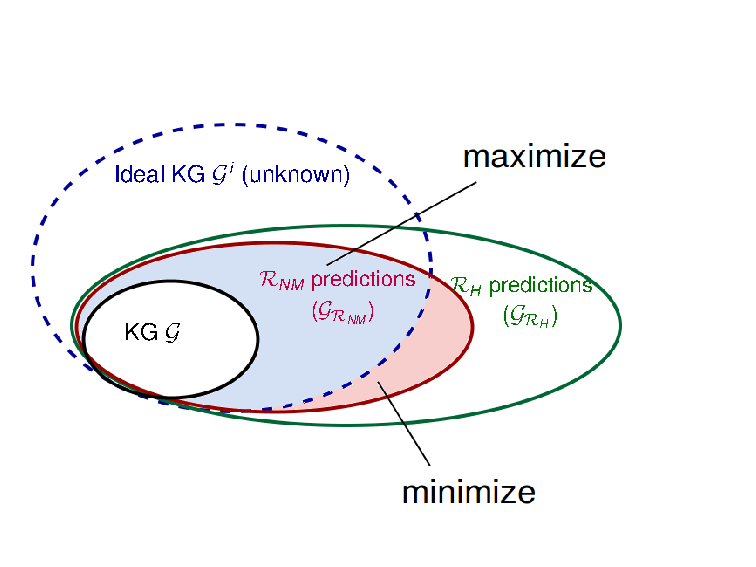
\includegraphics[width=0.55\textwidth]{big_pic}}
\end{picture}}

\only<2>{\vspace{-5.5cm}
\begin{beamerboxesrounded}[upper=uppercolgreen,lower=lowercolgreen,shadow=true]{Conflict is a constraint for a revision set with auxiliary rules}\bigskip

\small{$\alt<2>{\alert{\cR^{\mi{aux}}_{\mi{NM}}}}{\alert{\cR_{\mi{NM}}}}=\left\{
            \renewcommand{\arraystretch}{1.1}
             \begin{array}{@{\,}l@{~~}l@{}}
               \mi{\gr{r1:\,livesIn(X,Z) \leftarrow isMarriedTo(X,Y),livesIn(Y,Z),}} \\ \mi{\alert{\naf\ Researcher(X)}}\\
              \visible<2->{\mi{r1^{aux}:\,not\_livesIn(X,Z) \leftarrow isMarriedTo(X,Y),livesIn(Y,Z),} \\ \mi{Researcher(X)}\\}
              \mi{\gr{r2:\,livesIn(X,Z)\leftarrow workIn(X,Z),}\alert{\naf\ crossBorderWorker(X)}}\\
              \visible<2->{\mi{r2^{aux}:\,not\_livesIn(X,Z)}\leftarrow workIn(X,Z),crossBorderWorker(X)}
             \end{array}\right\}$\bigskip

possibly generate conflicting predictions $\{\gr{\mi{livesIn(a,b)},\mi{not\_livesIn(a,b)}}\}$~\cite{rumis} \bigskip

\textbf{Idea behind:} \alert{Researcher} is a good exception for \gr{$\mi{r1}$}, but the occurrence of \gr{$\mi{r2}$} might break this; conflicts should be minimized
}
\bigskip
\end{beamerboxesrounded}

}
\end{frame}

\begin{frame}\frametitle{Related Work}
\begin{itemize}
\item \textbf{\bl{Statistics-based Approaches}}
\medskip

\item \textbf{\bl{Logic-based Approaches}}
\begin{itemize}
\item ILP systems: ALEPH, QuickFOIL~\cite{quickfoil}
\item Relational learning systems: WARMR~\cite{warmr}, AMIE(+)~\cite{amie}, RDF2Rules~\cite{rdf2rules}
\item Nonmonotonic rule mining system~\cite{iswc2016}
\end{itemize}
\medskip


\item \textbf{\bl{Text-based Approaches}}
\medskip

\end{itemize}
\end{frame}


% \begin{frame}
% \begin{picture}(0.5,0.5)\put(0,-50){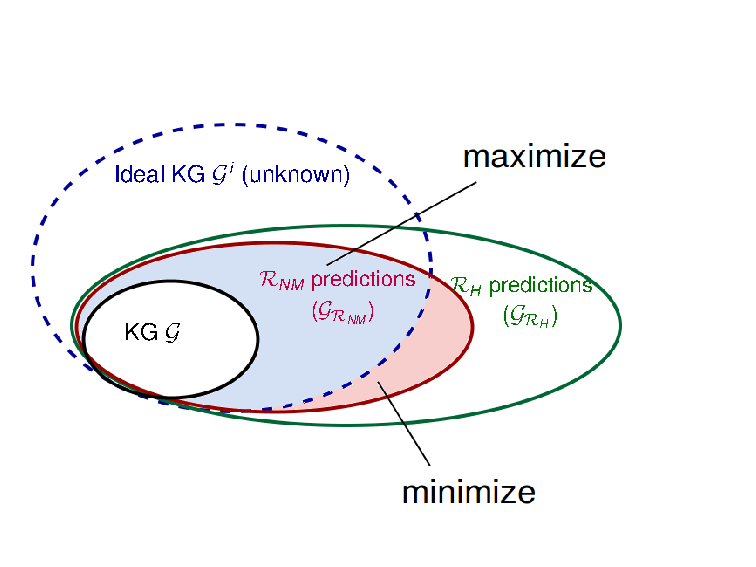
\includegraphics[width=0.85\textwidth]{big_pic}}\end{picture}
% \put(35,105){\hbox{\large{\bl{Ideal KG $\cG^i$ (unknown)}}}}
%   \put(45,39){\hbox{\large{KG $\cG$}}}
%  \put(100,55){\hbox{\alert{$\cR_{\mi{NM}}$ predictions}}}
%  \put(115,40){\hbox{\alert{($\cG_{\cR_{\mi{NM}}}$)}}}
%  \put(205,53){\hbox{\gr{$\cR_H$ predictions}}}
%  \put(227,38){\hbox{\large{\gr{($\cG_{\cR_H}$)}}}}
% \end{frame}
% \begin{frame}\frametitle{Quality-based Horn Theory Revision}

% \visible<3->{\bl{Goal:} revise a Horn ruleset \gr{$\cR_H$} mined from a KG $\cG$ to a nomonotonic \phantom{Goal: }one \alert{$\cR_{\mi{NM}}$} of a higher quality \wrt\ data prediction}

 
% \alt<5->{ \bigskip
%  \bigskip

% \small{$\alt<6>{\cR^{\mi{aux}}_{\mi{NM}}}{\alert{\cR_{\mi{NM}}}}=\left\{
%             \renewcommand{\arraystretch}{1.1}
%              \begin{array}{@{\,}l@{~~}l@{}}
%                \mi{\gr{r1:\,livesIn(X,Z) \leftarrow isMarTo(Y,X),livesIn(Y,Z),} \alert{\naf\ res(X)}}\\
%               \visible<6>{\mi{r1^{aux}:\,not\_livesIn(X,Z) \gr{\leftarrow isMarTo(Y,X),livesIn(Y,Z)},\alert{res(X)}}\\[3.45ex]}

%               \mi{\gr{r2:\,livesIn(X,Z)\leftarrow bornIn(X,Z),}\alert{\naf\ immigrant(X)}}\\
%               \visible<6>{\mi{r2^{aux}:\,not\_livesIn(X,Z)\gr{\leftarrow bornIn(X,Z)},\alert{immigrant(X)}}}
%              \end{array}\right\}$\bigskip
% \bigskip

% \visible<5->{\bl{$q_{\mi{rm}}(\cR_{\mi{NM}},\cG)$} computes average association rule measure \bl{$\mi{rm}$} for rules in $\cR_{\mi{NM}}$}
% \visible<6>{\medskip

% \bl{$q_{\mi{conflict}}(\cR_{\mi{NM}},\cG)$} estimates conflicting predictions made by $\cR^{\mi{aux}}_{\mi{NM}}$ on $\cG$\\${\{}\mi{\gr{livesIn(c,d)}{,}not\_livesIn(c,d)}{\}}$} 
% }
%         }{
%  \bigskip
%  \bigskip
%  \bigskip
%  \bigskip
%  \bigskip
%  \bigskip
%  \bigskip
%  \bigskip
%  \bigskip
%  \bigskip
%  \bigskip
%  \bigskip
%  \bigskip
%  \bigskip
%  \bigskip
%  \bigskip
%  \bigskip

% \alt<4>{\begin{picture}(0.5,0.5)\put(43,-5){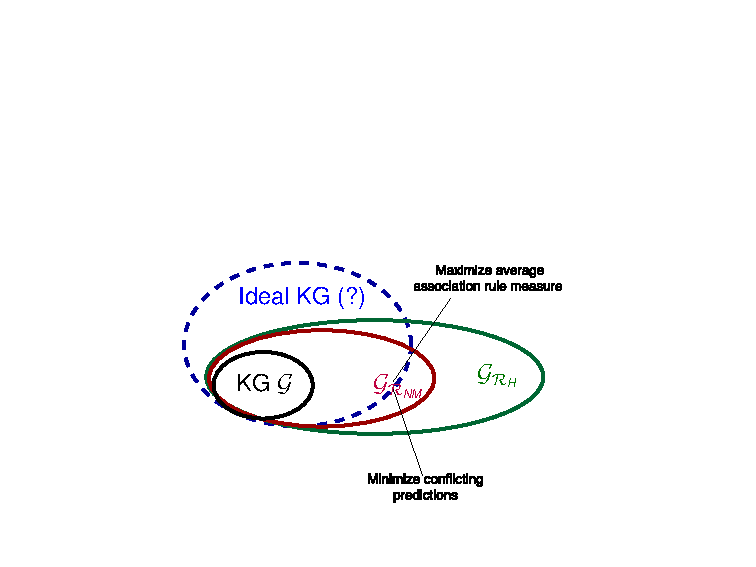
\includegraphics[width=0.85\textwidth]{step_5}}\end{picture}}{\alt<3>{\begin{picture}(0.5,0.5)\put(43,5){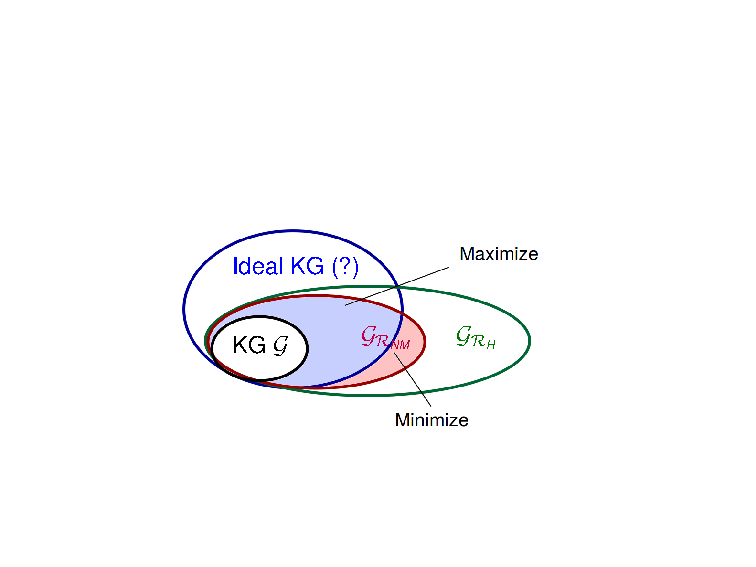
\includegraphics[width=0.85\textwidth]{big_picture}}\end{picture}}{\alt<2>{\begin{picture}(0.5,0.5)\put(43,10){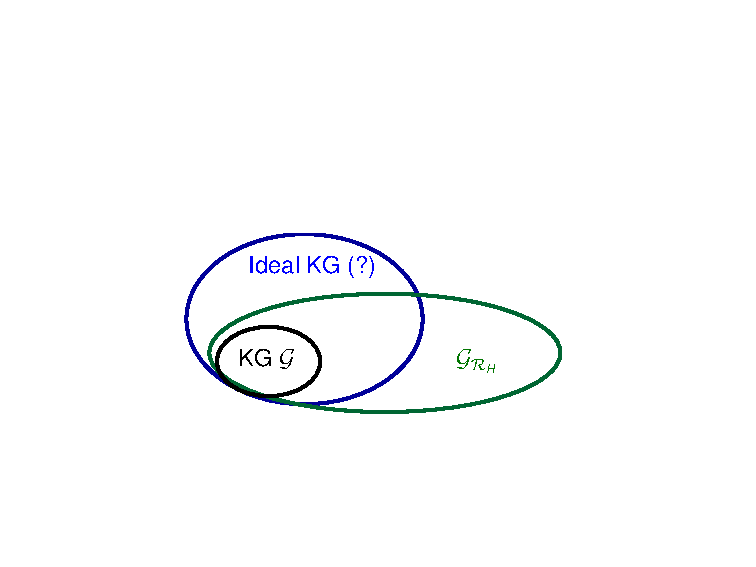
\includegraphics[width=0.85\textwidth]{step_2}}\end{picture}}{\begin{picture}(0.5,0.5)\put(43,15){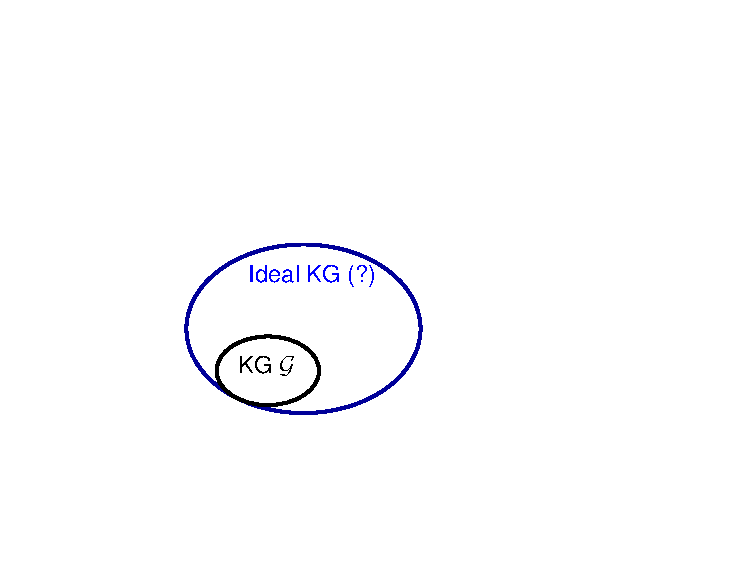
\includegraphics[width=0.57\textwidth]{step_1}}\end{picture}}}}}
% \end{frame}


 %\begin{frame}
 % \frametitle{Trial}
 % \begin{picture}(0.5,0.5)\put(73,-100){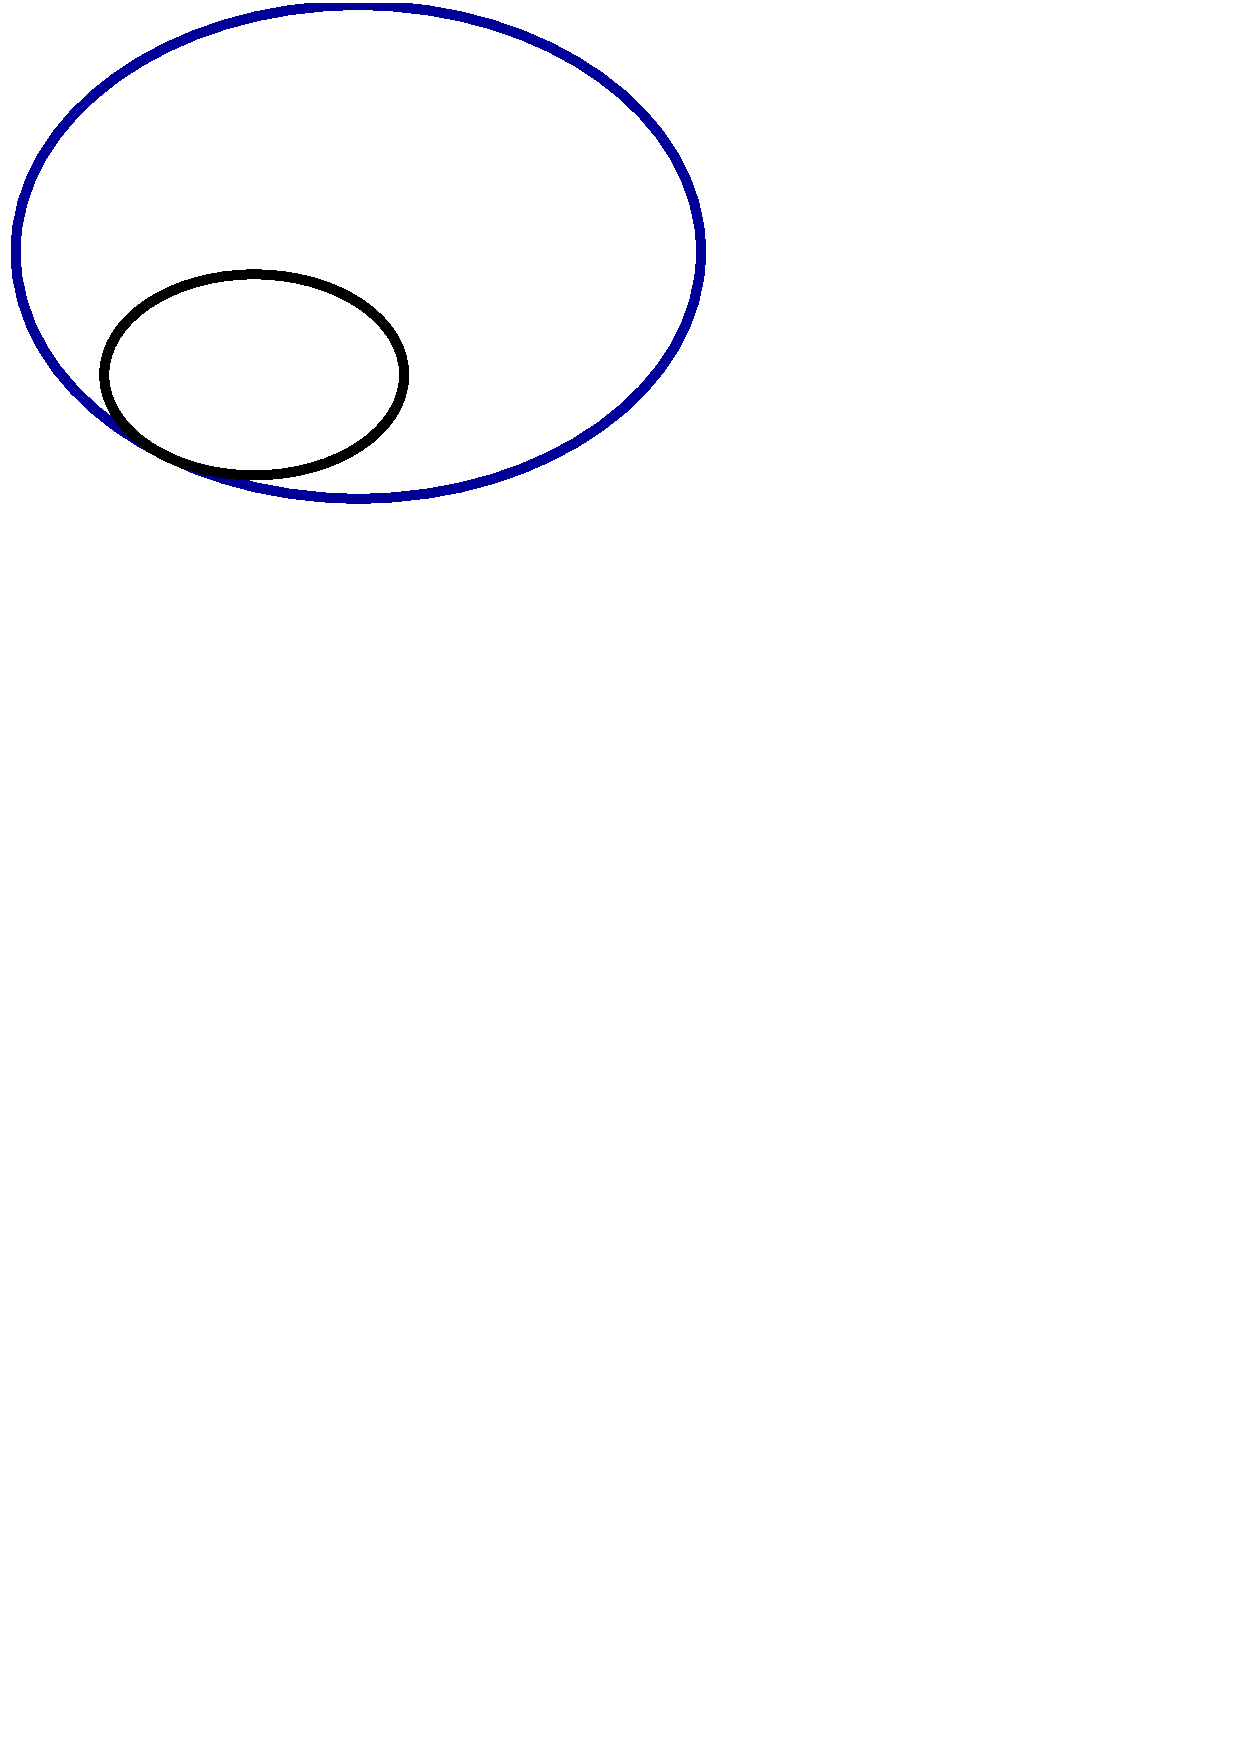
\includegraphics[width=0.35\textwidth]{big_picture_step_1}}\end{picture}
 %  \put(105,-35){\hbox{\large{\bl{Ideal KG (?)}}}}
 %  \put(100,-79){\hbox{\large{KG $\cG$}}}
 %  %\put(159,-58){\hbox{\large{\alert{$\cG_{\cR_{\mi{NM}}}$}}}}
 %  %\put(205,-58){\hbox{\large{\gr{$\cG_{\cR_{\mi{H}}}$}}}}
 % \end{frame}

% \begin{frame}
%  \frametitle{Trial}
%  \begin{picture}(0.5,0.5)\put(73,-100){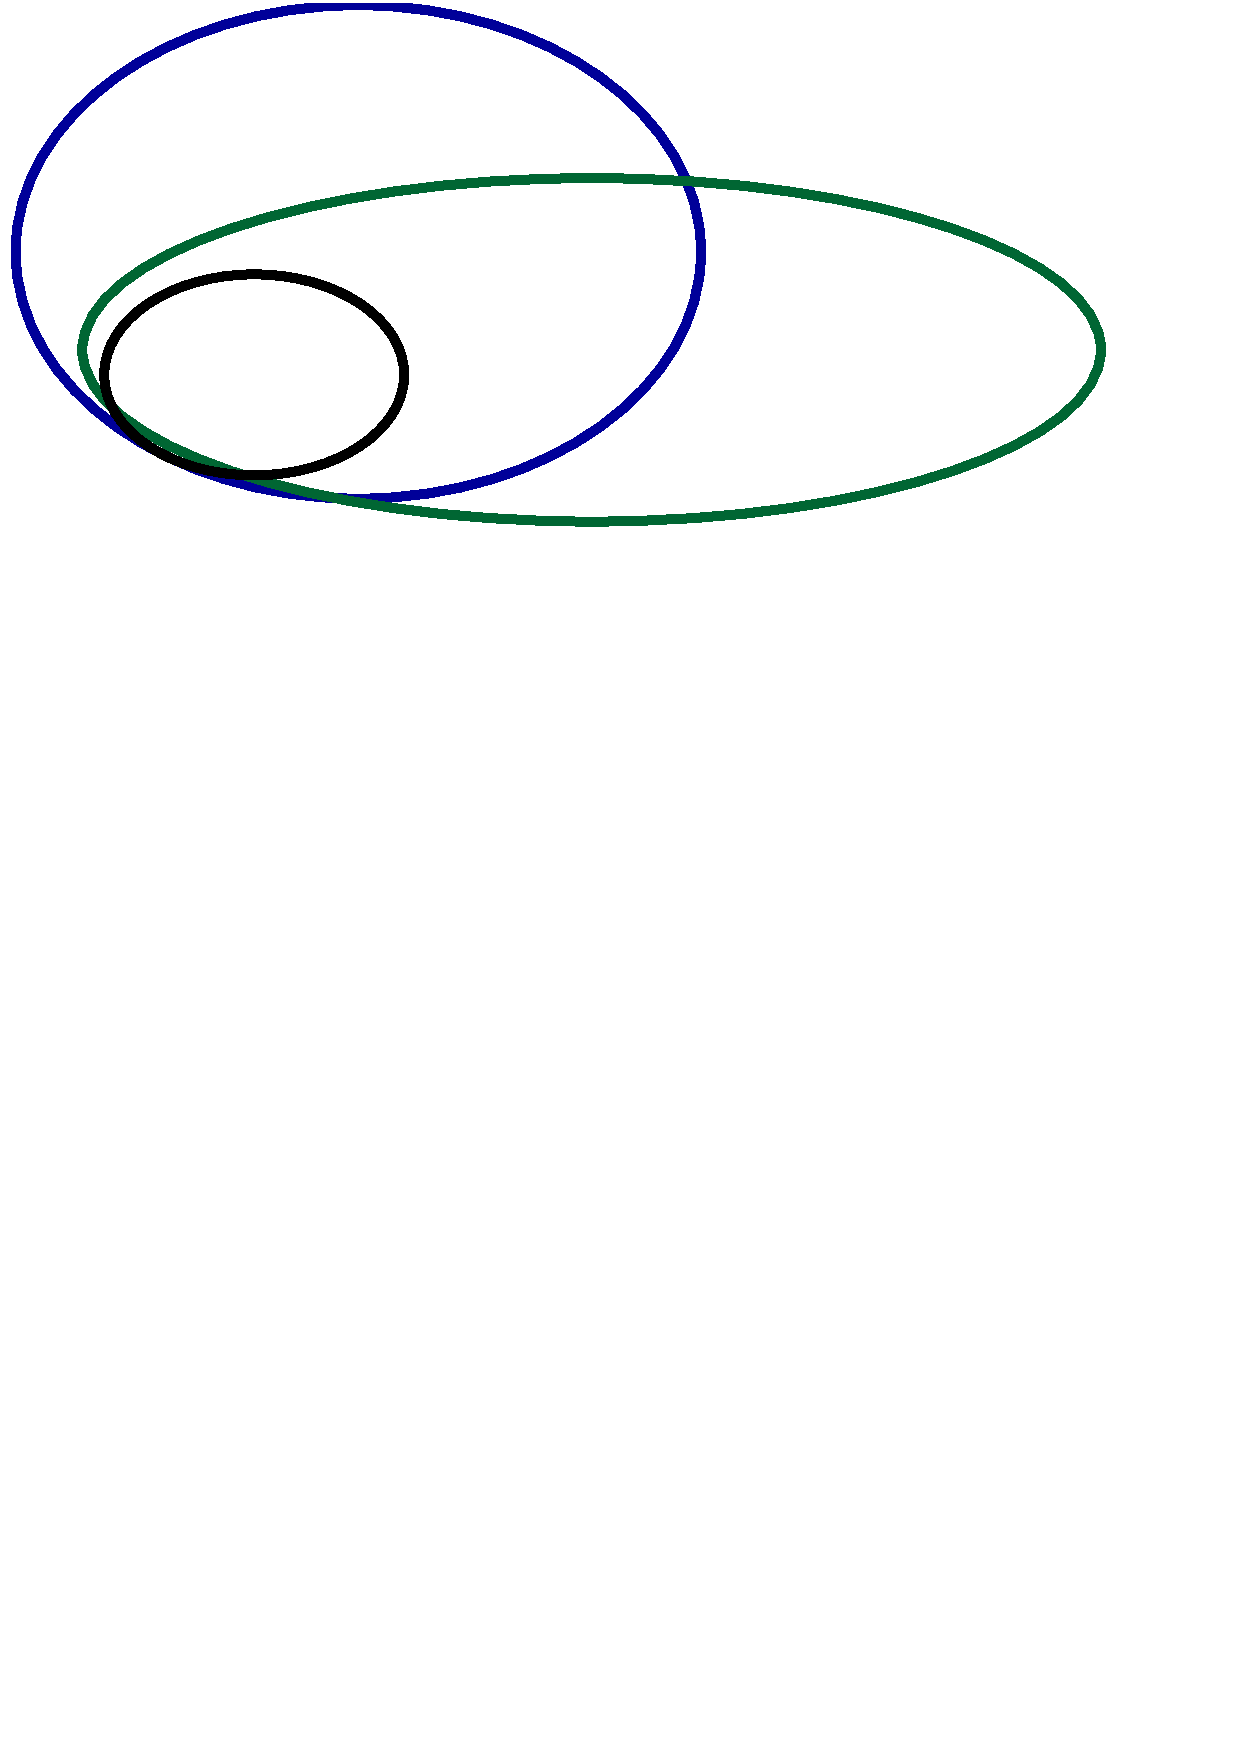
\includegraphics[width=0.55\textwidth]{big_picture_step_2}}\end{picture}
%   \put(105,-30){\hbox{\large{\bl{Ideal KG (?)}}}}
%   \put(100,-75){\hbox{\large{KG $\cG$}}}
%   %\put(159,-58){\hbox{\large{\alert{$\cG_{\cR_{\mi{NM}}}$}}}}
%   \put(205,-75){\hbox{\large{\gr{$\cG_{\cR_{\mi{H}}}$}}}}
%  \end{frame}

 % \begin{frame}
%   \frametitle{Trial}
%   \begin{picture}(0.5,0.5)\put(73,-150){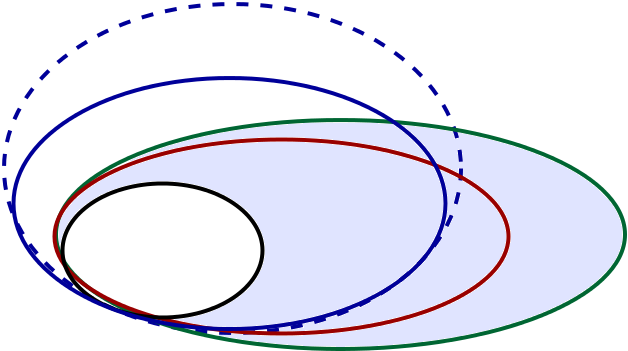
\includegraphics[width=0.55\textwidth]{R_H_all}}\end{picture}
%    \put(119,-65){\hbox{\large{\bl{$\cG^i$}}}}
%    \put(108,-83){\hbox{\large{\bl{$\cG^i_{\mi{appr}}$}}}}
%    \put(116,-125){\hbox{\large{$\cG$}}}
%    \put(165,-115){\hbox{\large{\alert{$\cG_{\cR_{\mi{NM}}}$}}}}
%    \put(227,-115){\hbox{\large{\gr{$\cG_{\cR_{\mi{H}}}$}}}}
%   \end{frame}

% \begin{frame}
%   \frametitle{Trial}
%   \begin{picture}(0.5,0.5)\put(73,-150){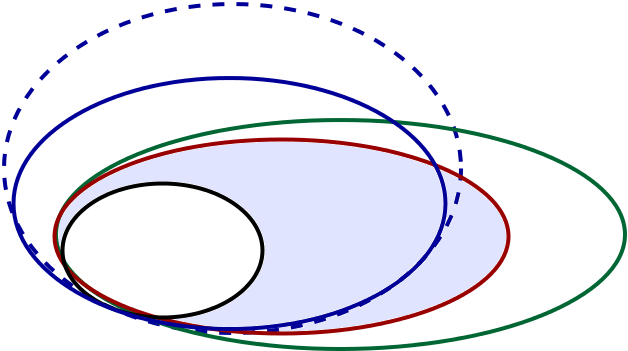
\includegraphics[width=0.55\textwidth]{R_NM_all}}\end{picture}
%    \put(119,-65){\hbox{\large{\bl{$\cG^i$}}}}
%    \put(108,-83){\hbox{\large{\bl{$\cG^i_{\mi{appr}}$}}}}
%    \put(116,-125){\hbox{\large{$\cG$}}}
%    \put(165,-115){\hbox{\large{\alert{$\cG_{\cR_{\mi{NM}}}$}}}}
%    \put(227,-115){\hbox{\large{\gr{$\cG_{\cR_{\mi{H}}}$}}}}
%   \end{frame}

% \begin{frame}
%   \frametitle{Trial}
%   \begin{picture}(0.5,0.5)\put(73,-150){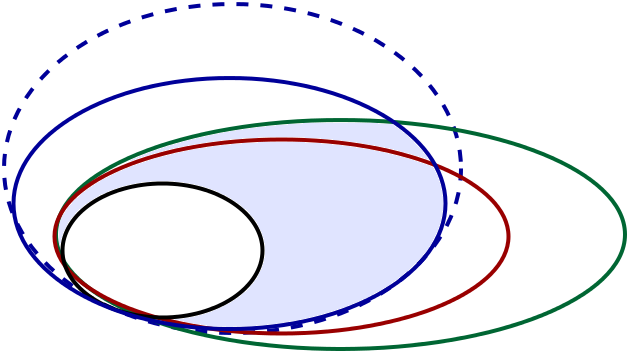
\includegraphics[width=0.55\textwidth]{R_H_Gi}}\end{picture}
%    \put(119,-65){\hbox{\large{\bl{$\cG^i$}}}}
%    \put(108,-83){\hbox{\large{\bl{$\cG^i_{\mi{appr}}$}}}}
%    \put(116,-125){\hbox{\large{$\cG$}}}
%    \put(165,-115){\hbox{\large{\alert{$\cG_{\cR_{\mi{NM}}}$}}}}
%    \put(227,-115){\hbox{\large{\gr{$\cG_{\cR_{\mi{H}}}$}}}}
%   \end{frame}

% \begin{frame}
%   \frametitle{Trial}
%   \begin{picture}(0.5,0.5)\put(73,-150){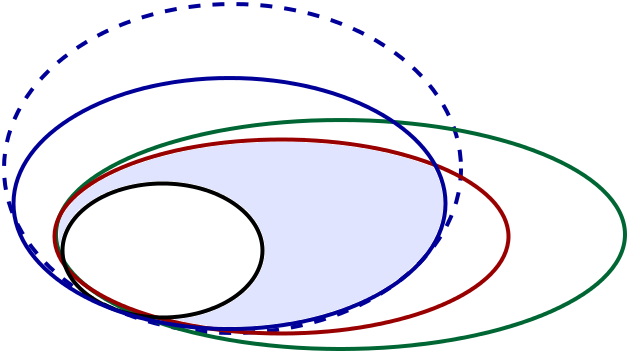
\includegraphics[width=0.55\textwidth]{R_NM_Gi}}\end{picture}
%    \put(119,-65){\hbox{\large{\bl{$\cG^i$}}}}
%    \put(108,-83){\hbox{\large{\bl{$\cG^i_{\mi{appr}}$}}}}
%    \put(116,-125){\hbox{\large{$\cG$}}}
%    \put(165,-115){\hbox{\large{\alert{$\cG_{\cR_{\mi{NM}}}$}}}}
%    \put(227,-115){\hbox{\large{\gr{$\cG_{\cR_{\mi{H}}}$}}}}
%   \end{frame}

% \begin{frame}
%   \frametitle{Trial}
%   \begin{picture}(0.5,0.5)\put(73,-150){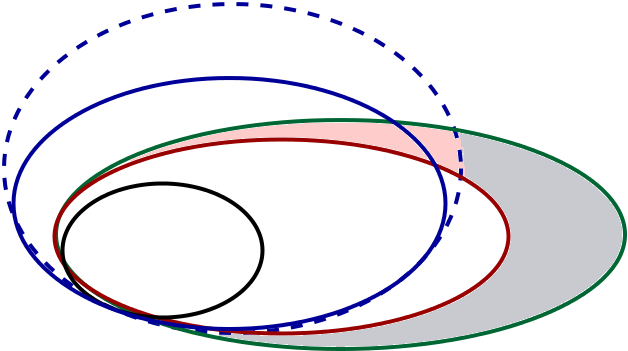
\includegraphics[width=0.55\textwidth]{R_NM_negl_corr_incorr}}\end{picture}
%    \put(119,-65){\hbox{\large{\bl{$\cG^i$}}}}
%    \put(108,-83){\hbox{\large{\bl{$\cG^i_{\mi{appr}}$}}}}
%    \put(116,-125){\hbox{\large{$\cG$}}}
%    \put(165,-115){\hbox{\large{\alert{$\cG_{\cR_{\mi{NM}}}$}}}}
%    \put(227,-115){\hbox{\large{\gr{$\cG_{\cR_{\mi{H}}}$}}}}
%   \end{frame}



%\makeoverview
\section{RUMIS System}


\begin{frame}\frametitle{RUMIS Architecture}

\bigskip
We develop a nonmonotonic \textbf{RU}le \textbf{MI}ning \textbf{S}ystem in the relational setting
\smallskip

\begin{figure}[h]
	\centering
	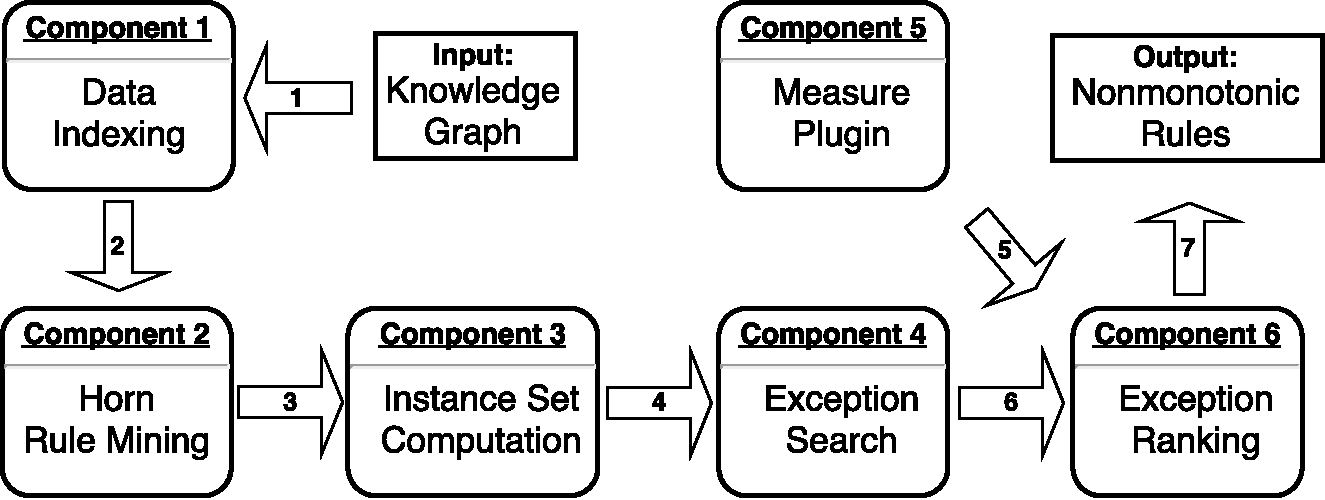
\includegraphics[page=1,width=.75\textwidth]{system_overview.pdf}
	\caption{Components of RUMIS}
\end{figure}

\end{frame}

\begin{frame}{Data Indexing}

\textbf{Goal:} support searching over a dataset
\smallskip

\textbf{Intuition:} 
\begin{itemize}
	\item Inverted indexing from term to document in IR systems
  	\item In this problem, a triple is a document
  	\item Find corresponding predicates given subject, object
\end{itemize}

\begin{figure}[h]
	\centering
	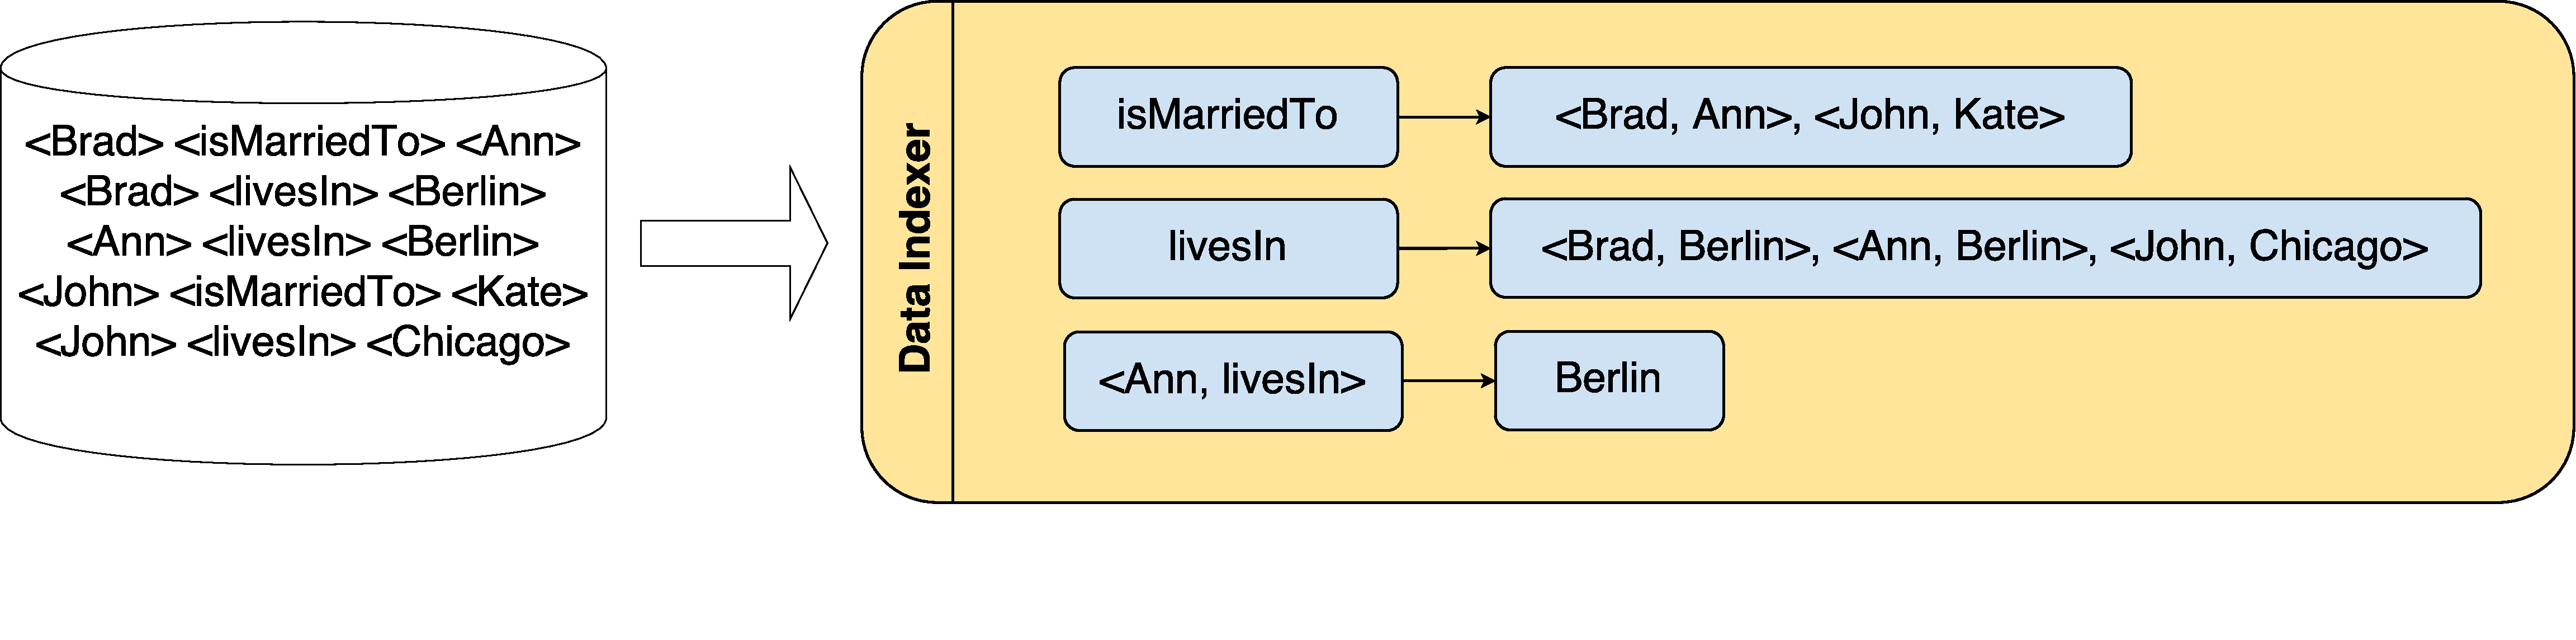
\includegraphics[page=1,width=1.0\textwidth]{data_indexing.pdf}
	\caption{Data Indexing Component}
\end{figure}

\end{frame}

\begin{frame}{Horn Rule Mining}

\textbf{Given:} KG $\cG$
\smallskip

\textbf{Find:} Horn rules \textit{\textbf{h(X, Z) $\leftarrow$ p(X, Y), q(Y, Z)}}
\smallskip
\begin{itemize}
	\item Simplify \textit{language bias} challenge
	\item $asupp(r)=|\{(X/a, Y/b, Z/c):h(a, c),p(a, b),q(b, c)\}|$
	\item Top rules with the highest $asupp$ are computed using Data Indexer
	\item Another tool can be used in this step
\end{itemize}

\end{frame}

\begin{frame}{Instance Set Computation}

\smallskip
Consider the rule \textcolor{darkgreen}{\textit{livesIn(X,Z) $\leftarrow$ isMarriedTo(X,Y),livesIn(Y,Z)}}

\smallskip
\only<1>{
Its normal set is \textit{$\langle$Brad, Berlin$\rangle$}, \textit{$\langle$John, Chicago$\rangle$}, \textit{$\langle$Sue, Beijin$\rangle$}

\smallskip

\begin{figure}[h]
	\centering
	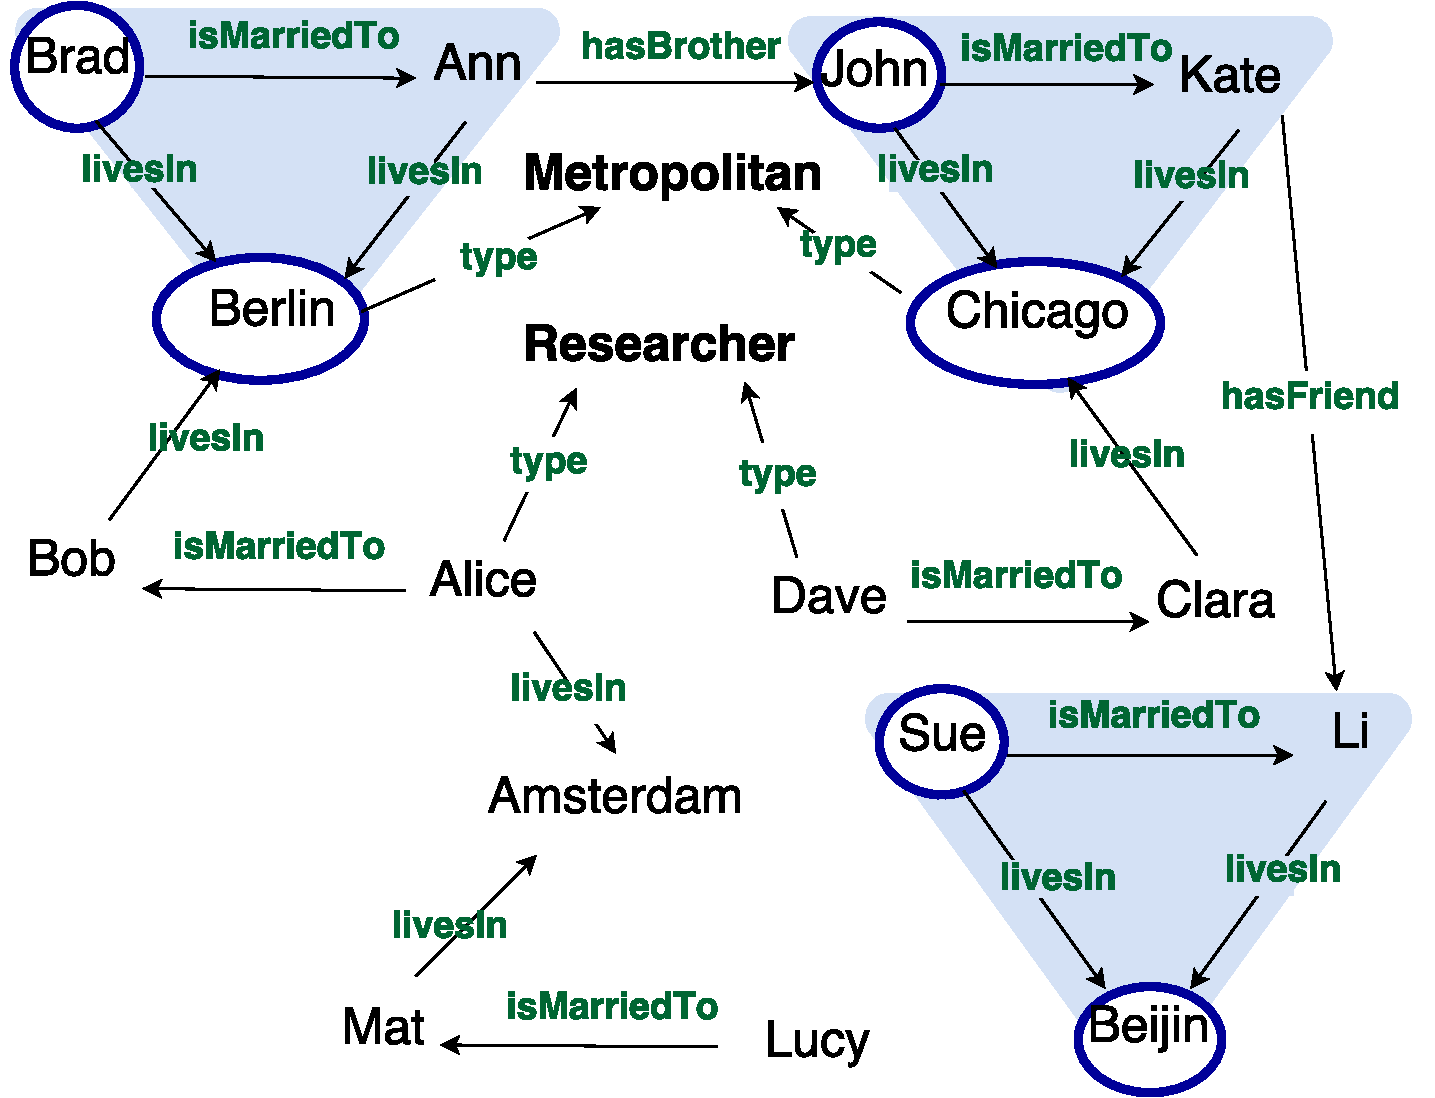
\includegraphics[page=1,width=0.65\textwidth]{kg_advanced_col_1.pdf}
	\caption{A normal set example~\cite{rumis}}
\end{figure}
}

\only<2>{
Its abnormal set is \textit{$\langle$Alice, Berlin$\rangle$}, \textit{$\langle$Dave, Chicago$\rangle$}, \textit{$\langle$Lucy, Beijin$\rangle$}

\smallskip

\begin{figure}[h]
	\centering
	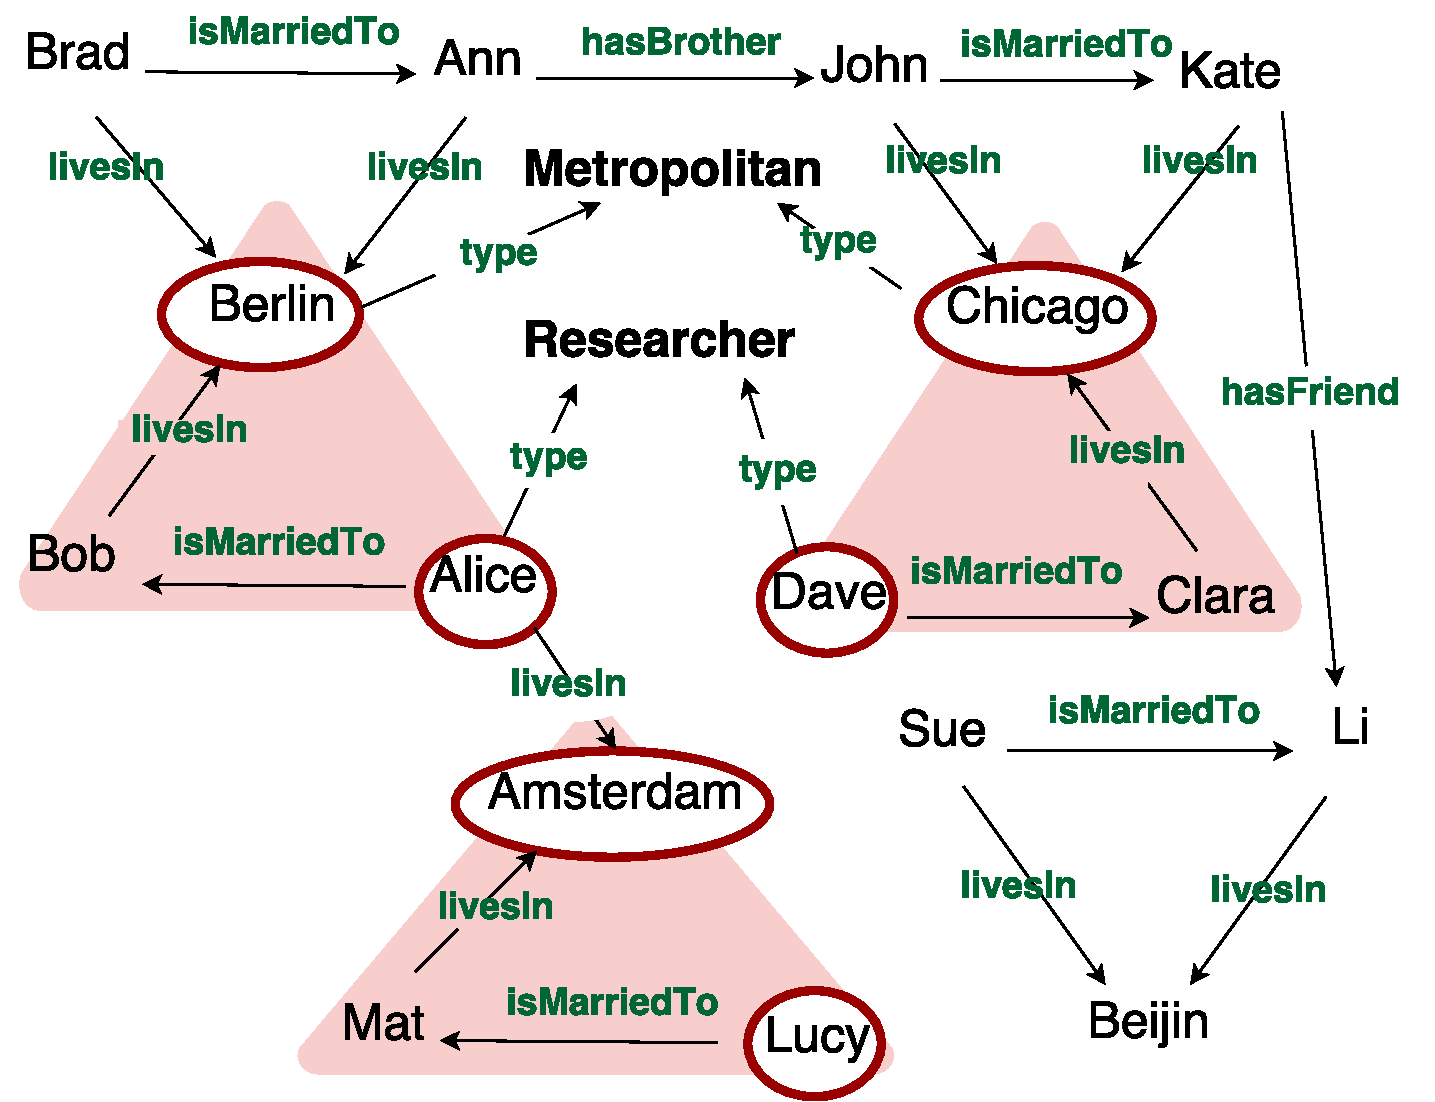
\includegraphics[page=1,width=0.65\textwidth]{kg_advanced_col_2.pdf}
	\caption{An abnormal set example~\cite{rumis}}
\end{figure}
}

\end{frame}

\begin{frame}{Instance Set Computation}

\bigskip
\textbf{Given:} KG $\cG$, Horn rules \textit{\textbf{h(X, Z) $\leftarrow$ p(X, Y), q(Y, Z)}}

\smallskip
\textbf{Goal:} Find (ab)normal sets exploiting Data Indexer
\begin{itemize}
	\item Traverse all substitutions for $X$.
	\item Find list of $Y$ from $pX$ based on indexing.
	\item Find list of $Z$ from $qY$ based on indexing.
	\item Check \textit{$\langle$X h Z$\rangle$} in the graph or not.
	\item Classify \textit{$\langle$X Z$\rangle$} into $NS(r)$ and $ABS(r)$.
\end{itemize}

\end{frame}

% \begin{frame}\frametitle{Step 1: Mine Horn Rules}
% \begin{picture}(0.5,0.5)\put(53,-193){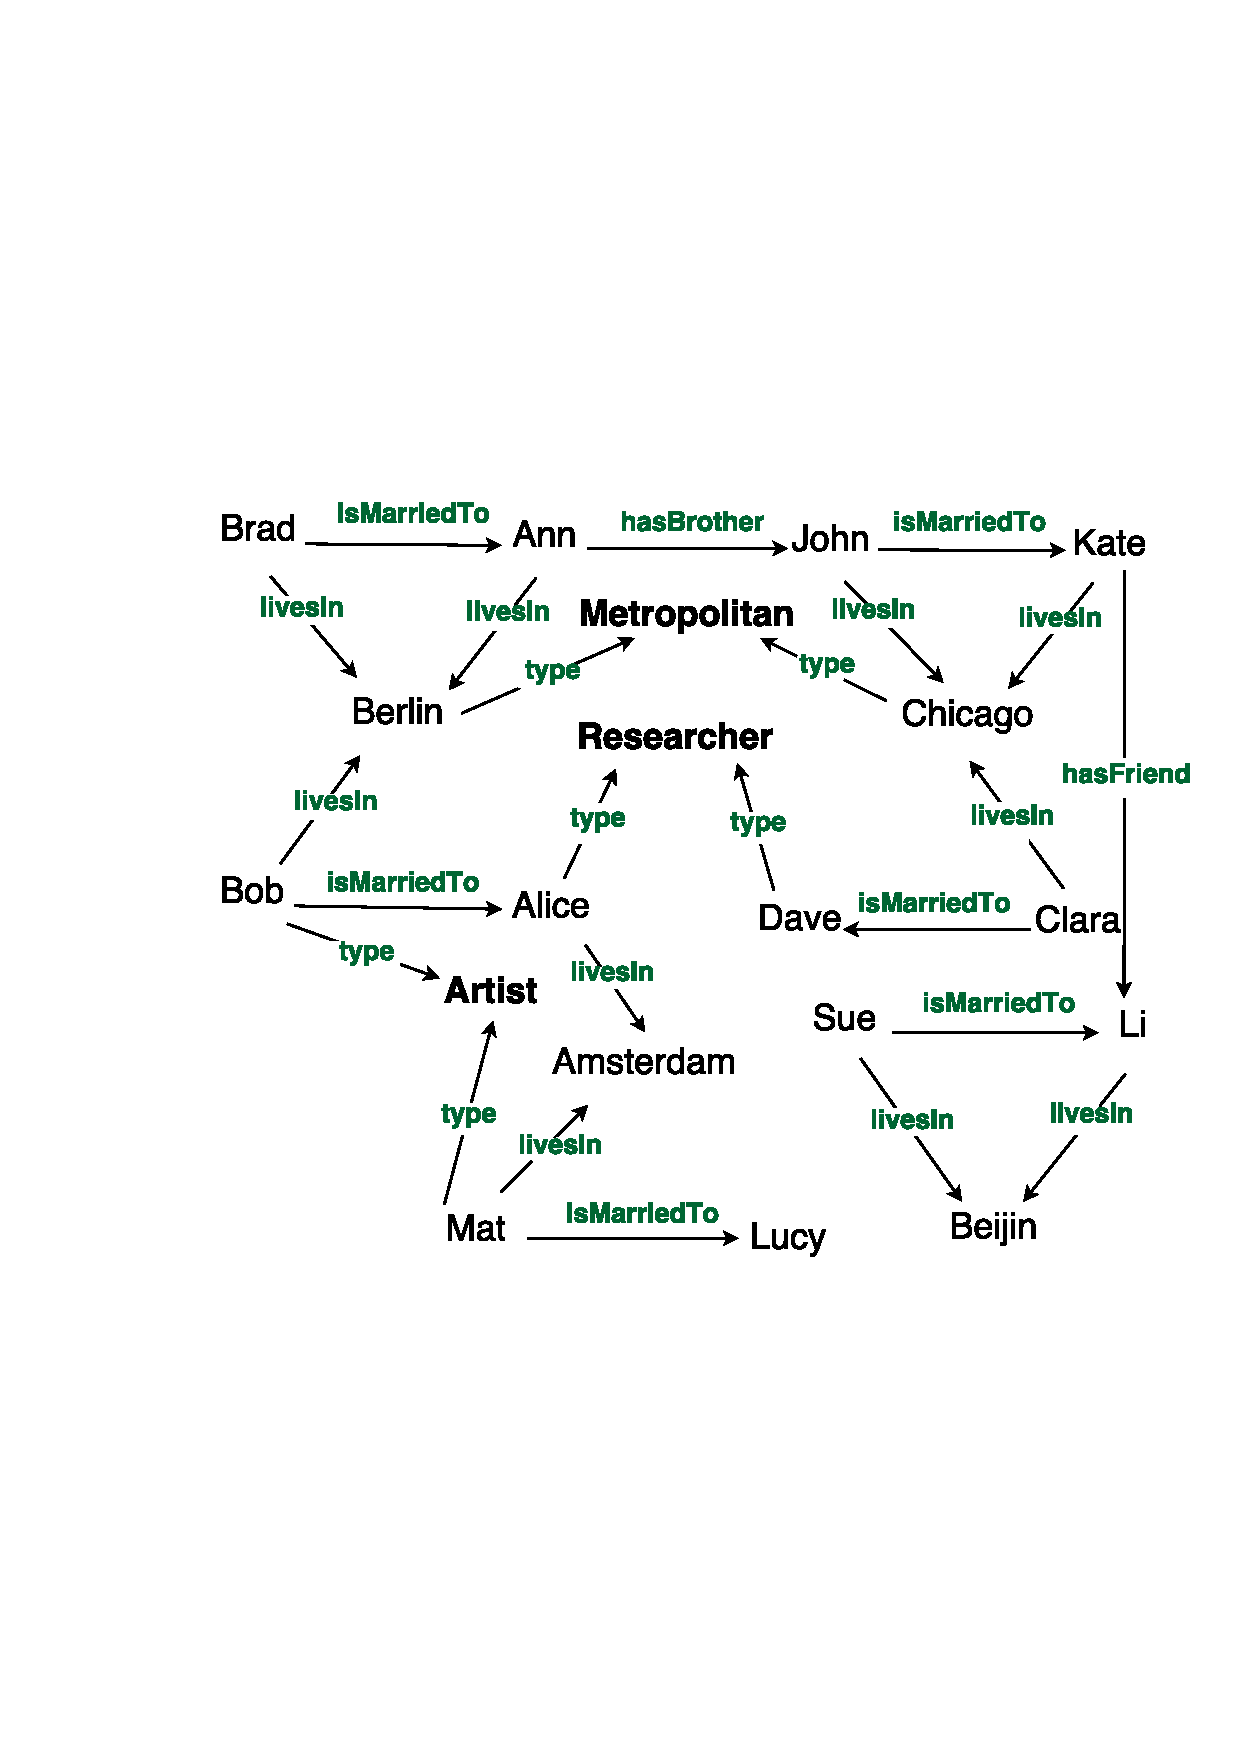
\includegraphics[width=0.75\textwidth]{kg_advanced_1}}\end{picture}
% \bigskip
% \bigskip
% \bigskip
% \bigskip
% \bigskip
% \bigskip
% \bigskip
% \bigskip
% \bigskip
% \bigskip
% \bigskip
% \bigskip
% \bigskip
% \bigskip
% \bigskip
% \bigskip
% \bigskip

% \centerline{\textcolor{darkgreen}{$\mi{r:\;livesIn(X,Z)}\leftarrow \mi{isMarriedTo(Y,X),livesIn(Y,Z)}$}}

% \end{frame}
\begin{frame}\frametitle{Exception Search}
\begin{picture}(0.5,0.5)\put(55,-195){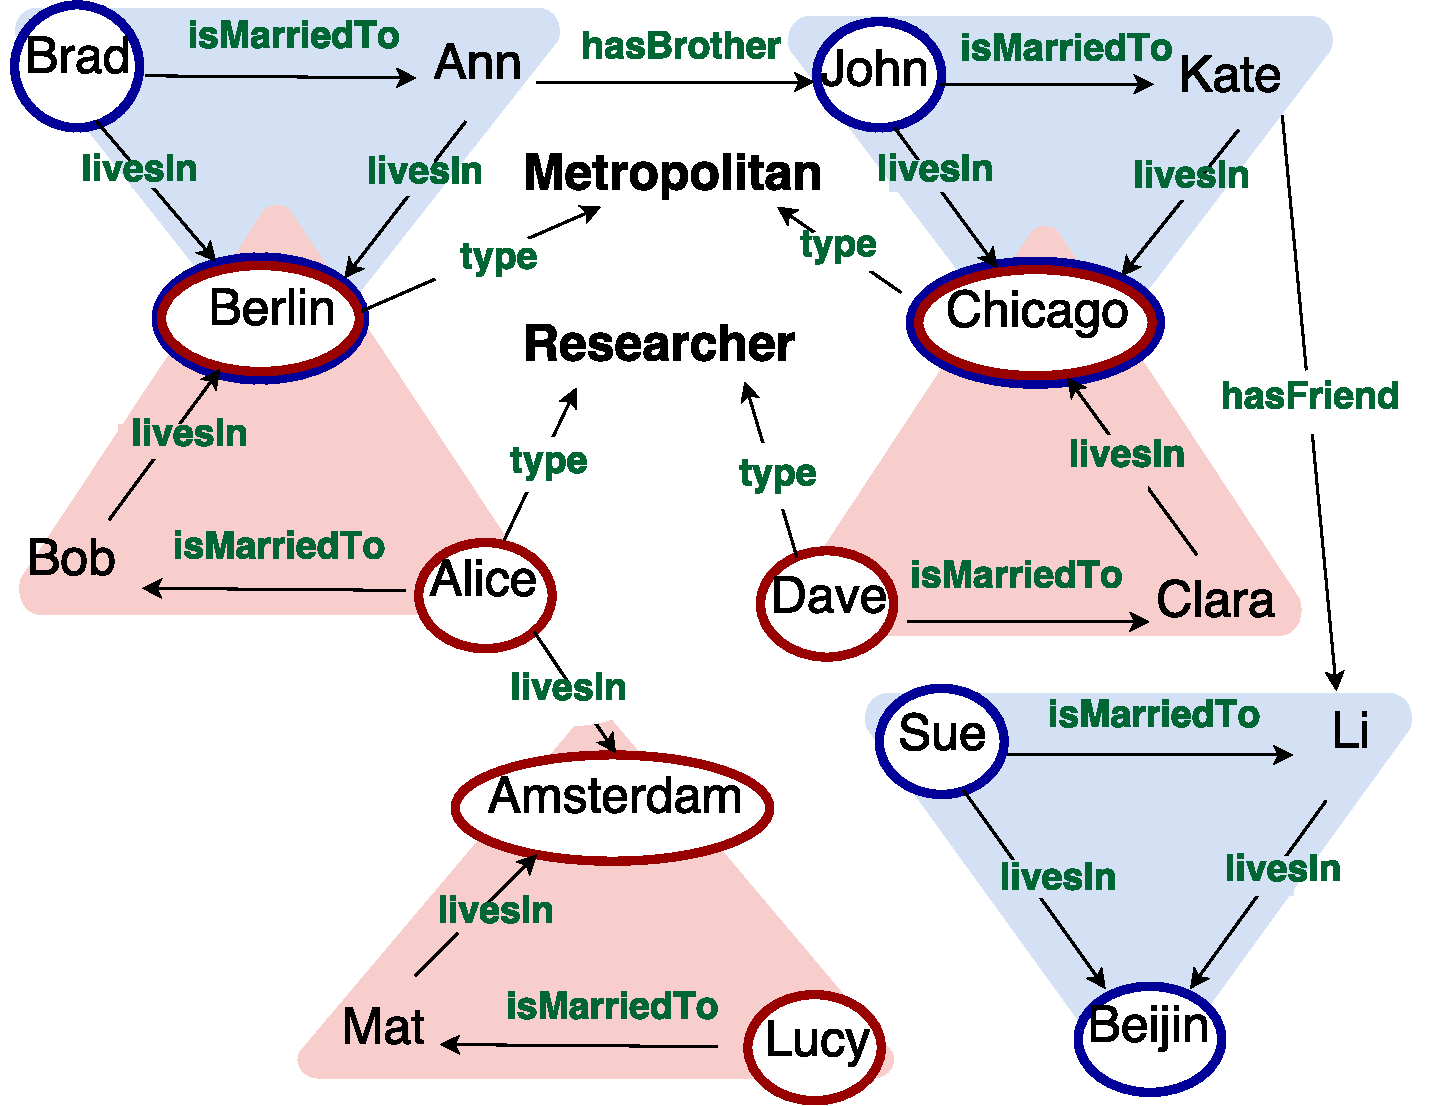
\includegraphics[width=0.65\textwidth]{kg_advanced_col}}
\end{picture}
\bigskip
\bigskip
\bigskip
\bigskip
\bigskip
\bigskip
\bigskip
\bigskip
\bigskip
\bigskip
\bigskip
\bigskip
\bigskip
\bigskip
\bigskip
\bigskip
\bigskip


\centerline{\textcolor{darkgreen}{\textit{r: \textit{livesIn(X,Z)} $\leftarrow$ isMarriedTo(X, Y), livesIn(Y, Z), not Researcher(X)}}}

\end{frame}



\begin{frame}\frametitle{Exception Ranking}

\begin{center}
$\gr{\mi{r1} \dotsc \dotsc \dotsc} \{\alert{\underline{\mathbf{e_1}},e_2,e_3, \dotsc}\}$\\
 $\gr{\mi{r2} \dotsc \dotsc \dotsc} \{\alert{e_1,\underline{\mathbf{e_2}},e_3, \dotsc}\}$\\
 $\gr{\mi{r3} \dotsc \dotsc \dotsc} \{\alert{\underline{\mathbf{e_1}},e_2,e_3, \dotsc}\}$\\
\end{center}
\bigskip
\begin{beamerboxesrounded}[upper=uppercolred,lower=lowercolred,shadow=true]{}
Finding global optimum solution for QHTR is impracticable
\end{beamerboxesrounded}
\begin{itemize}
\item \bl{Naive ranking:} among all revisions of $r\in \cR_{H}$, $r'$ having the largest $\mi{conv}(r,\cG)$ is chosen

\bigskip
\bigskip

\item \bl{Partial Materialization (PM):} for each rule $r$, KG $\cG'$ includes $\cG$ and predicted facts of other rules. PM selects a revision having the largest $\dfrac{\mi{conv(r,\cG')+conv(r^{aux},\cG')}}{2}$

% \only<2>{
% $\gr{r1 \dotsc \dotsc \dotsc} \{\alert{\underline{\mathbf{e_1}},e_2,e_3, \dotsc}\}$\\
% \hilight{$\gr{r2 \dotsc \dotsc \dotsc} \{\alert{e_1,e_2,e_3, \dotsc}\}$\\
% $\gr{r3 \dotsc \dotsc \dotsc} \{\alert{e_1,e_2,e_3, \dotsc}\}$\\}}

\bigskip
\bigskip

\item \bl{Ordered Partial Materialization (OPM):} similar to PM, but only previous rules of $r$ are used to predict new facts
\end{itemize}

\end{frame}

\section{Experiments}
\begin{frame}\frametitle{Preliminary Experiments}
\begin{itemize}
\item \bl{$\cG^i_{\mi{appr}}$}: IMDB (movie) KG\footnote{\url{http://imdb.com}}: $\approx$ 600.000 facts, $\approx$ 40 relations
\begin{itemize}
\item[] E.g., $\gr{\mi{directedBy}}$, $\gr{\mi{actedIn}}$
\end{itemize}
\medskip

\item \bl{$\cG$}: random. rem. 20\% from $\cG^i_{\mi{appr}}$ for every relation
\medskip

\item \bl{$\cR_H$}: $\mi{h(X,Y)\leftarrow p(X,Z),q(Z,Y)}$ mine from $\cG$
\medskip

\item \bl{Exception types}: $\mi{e_1(X),e_2(Y),e_3(X,Y)}$
\medskip

\item \bl{OPM} ranker, predictions are computed by \bl{answer set solver} dlv\footnote{\url{http://dlvsystem.com}}
%\item $\bl{\mi{rm}}$ measure: $\mi{conv(r)=\dfrac{1-supp(r)}{1-conf(r)}}$
\end{itemize}

% \alt<6->{\begin{picture}(0.5,0.5)\put(93,-53){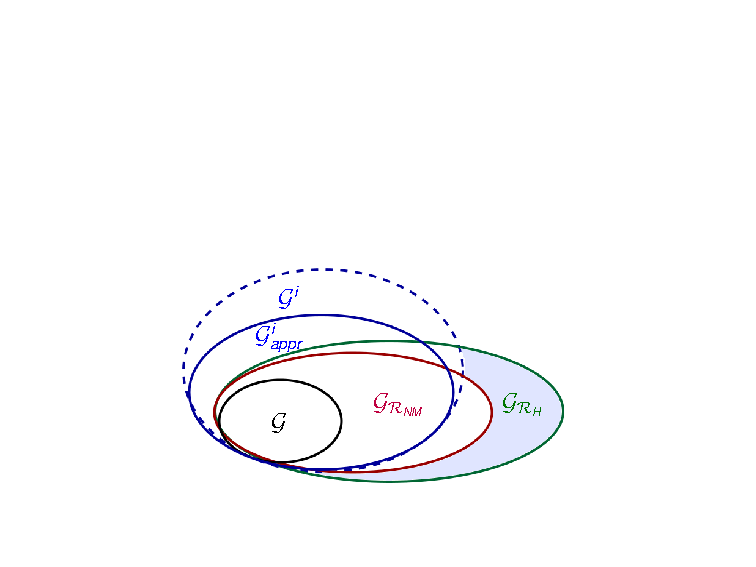
\includegraphics[width=0.45\textwidth]{exp_nm_negl}}\end{picture}}{\alt<5->{\begin{picture}(0.5,0.5)\put(93,-53){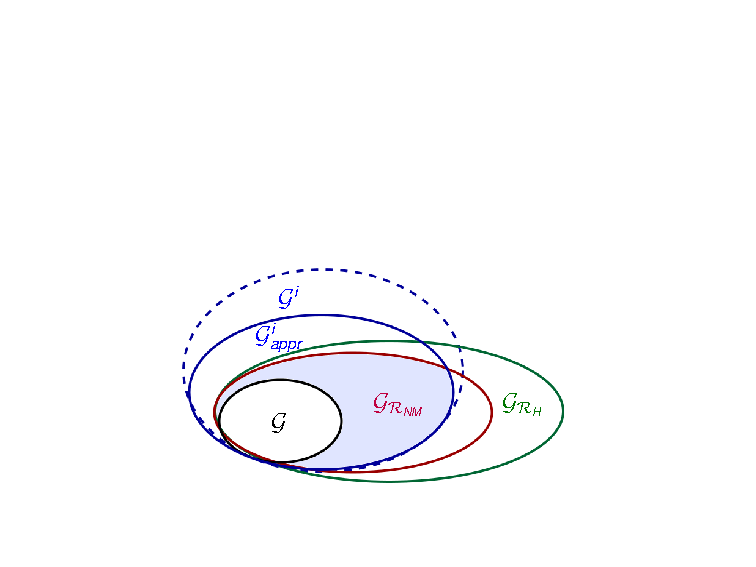
\includegraphics[width=0.45\textwidth]{exp_nm_gi}}\end{picture}}{\alt<4->{\begin{picture}(0.5,0.5)\put(93,-53){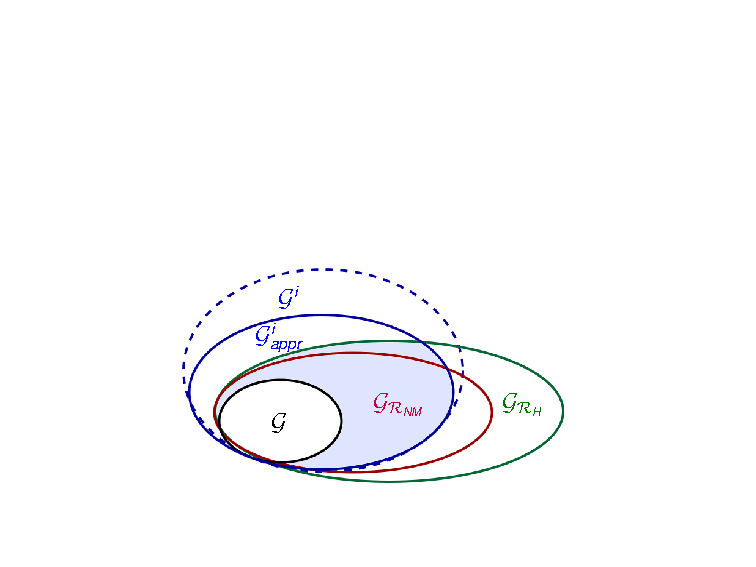
\includegraphics[width=0.45\textwidth]{exp_horn_gi}}\end{picture}}{\alt<3->{\begin{picture}(0.5,0.5)\put(93,-53){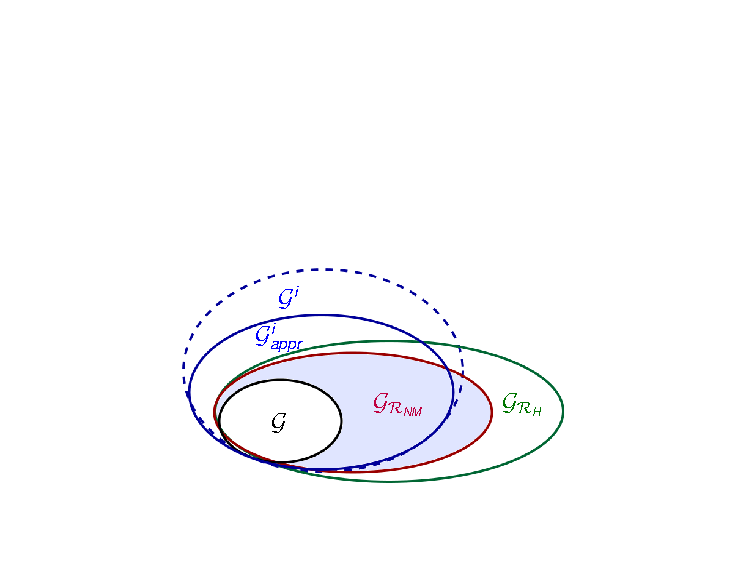
\includegraphics[width=0.45\textwidth]{exp_nm_all}}\end{picture}}{\begin{picture}(0.5,0.5)\put(93,-53){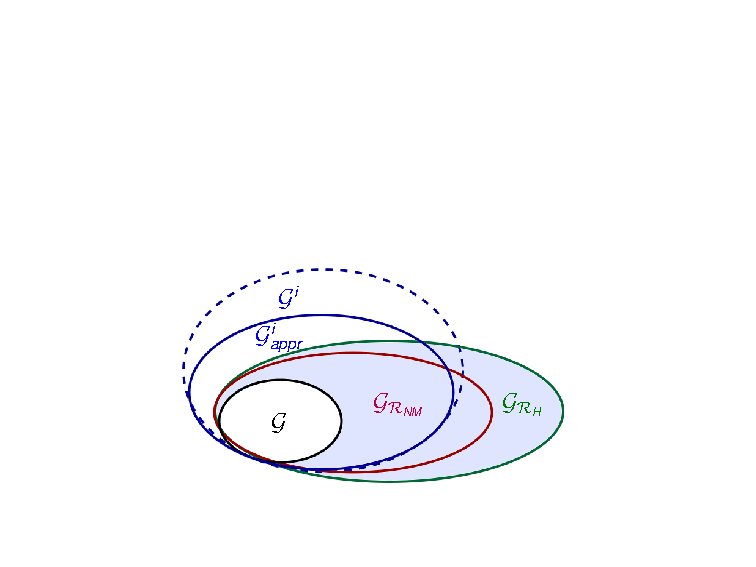
\includegraphics[width=0.45\textwidth]{exp_horn_all}}\end{picture}
% }}}}}
\end{frame}


\begin{frame}\frametitle{Preliminary Experiments}
\only<1>{\vspace{-1.4cm}}
\centering
\begin{table}[]
\scriptsize
\begin{tabular}{|r|r|r|r|r|r|r|r|r|r|}
\hline
\multicolumn{1}{|c|}{\multirow{3}{*}{\textbf{k}}} & \multicolumn{2}{c|}{\multirow{2}{*}{\textbf{avg. conv.}}}            & \multicolumn{1}{c|}{\multirow{2}{*}{\textbf{confl.}}} & \multicolumn{6}{c|}{\textbf{number of predictions}}                                                                                                                                                                                                           \\ \cline{5-10} 
\multicolumn{1}{|c|}{}                            & \multicolumn{2}{c|}{}                                                & \multicolumn{1}{c|}{}                                 & \multicolumn{2}{c|}{\textbf{$\cR_{\mi{H}}$}}                                           & \multicolumn{2}{c|}{\textbf{$\cR_{\mi{NM}}$}}                                          & \multicolumn{2}{c|}{\textbf{$\cR_{\mi{H}}$ not $\cR_{\mi{NM}}$}}                                                        \\ \cline{2-10} 
\multicolumn{1}{|c|}{}                            & \multicolumn{1}{c|}{\textbf{$\cR_{\mi{H}}$}} & \multicolumn{1}{c|}{\textbf{$\cR_{\mi{NM}}$}} & \multicolumn{1}{c|}{\textbf{$\cR_{\mi{NM}}$}}                     & \multicolumn{1}{c|}{\textbf{all}} & \multicolumn{1}{c|}{\textbf{in $\cG_{\mi{appr}}^i$}} & \multicolumn{1}{c|}{\textbf{all}} & \multicolumn{1}{c|}{\textbf{in $\cG_{\mi{appr}}^i$}} & \multicolumn{1}{c|}{\textbf{false} $\checkmark$} & \multicolumn{1}{c|}{\textbf{in $\cG_{\mi{appr}}^i$}} \\ \hline
5                                                 & 4.08                             & 6.16                              & 0.28                                                  & 345                               & 161                                    & 331                               & \hilightbl{156}                                    & \hilightgray{0}                                                  & \hilightgreen{14}                                             \\
10                                                & 2.91                             & 4.21                              & 0.08                                                  & 2178                              & 456                                    & 2118                              & \hilightbl{450}                                    & \hilightgray{27}                                                 & \hilightgreen{33}                                             \\
15                                                & 2.5                              & 3.42                              & 0.09                                                  & 3482                              & 629                                    & 3348                              & \hilightbl{622}                                    & \hilightgray{86}                                                 & \hilightgreen{48}                                             \\
20                                                & 2.29                             & 3.0                               & 0.13                                                  & 5278                              & 848                                    & 5046                              & \hilightbl{835}                                    & \hilightgray{157}                                               & \hilightgreen{75}                                            
\\ \hline
\end{tabular}
\smallskip

\caption{Top $k$ rule revision results}

\end{table}

\alt<2>{ \textbf{\bl{Examples of revised rules:}}\bigskip

 \begin{tabular}{l}
 {\footnotesize
        %\multirow{6}{*}{YAGO $\begin{cases} \\ \\ \end{cases}$}
        $\gr{r_1:  \mi{writtenBy(X, Z)}  \leftarrow
        \mi{hasPredecessor(X, Y)},\mi{writtenBy(Y, Z)},}$ \alert{$ \textbf{not}$  $\mi{is\_American\_film(X)} $}}\\        
       {\footnotesize 
$\gr{r_2:  \mi{actedIn(X, Z)}  \leftarrow
        \mi{isMarriedTo(X, Y)},\mi{directed(Y, Z)},}$ \alert{$ \textbf{not}$  $\mi{is\_silent\_film\_actor(X)} $}} \\
    
 \end{tabular}            
  }{\begin{picture}(0.5,0.5)\put(-83,-75){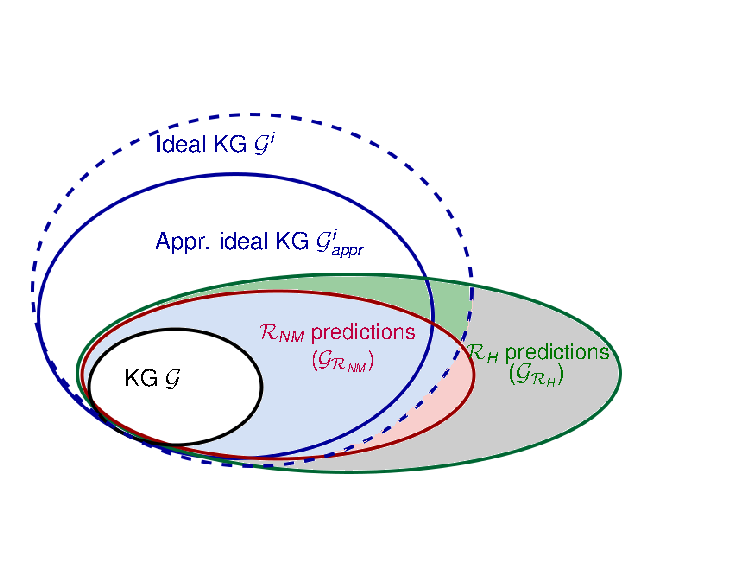
\includegraphics[width=0.56\textwidth]{big_pic_exp}}\end{picture}}

\end{frame}

% \begin{frame}\frametitle{Preliminary Experiments}
% \vspace{-1.7cm}
% \begin{table}[t]
% \centering
% \footnotesize
% \renewcommand*{\arraystretch}{1.07}
% \begin{tabular}{|r|r|r|r|r|r|r|r|r|}
% \hline
% \multicolumn{1}{|c|}{\multirow{3}{*}{\,\bf{$k$}\,}} & \multicolumn{2}{c|}{\multirow{2}{*}{\bf{avg. conv.}}}    & \multicolumn{1}{c|}{\multirow{2}{*}{\bf{confl.}}} & \multicolumn{5}{c|}{\bf{number of predictions}}                                                                                                            \\ \cline{5-9} 
% \multicolumn{1}{|c|}{}                         & \multicolumn{2}{c|}{}                               & \multicolumn{1}{c|}{}                        & \multicolumn{2}{c|}{\bf{all}}                            & \multicolumn{2}{c|}{\bf{in $\cG^i_{\mi{appr}}$}}                     & \multicolumn{1}{c|}{\bf{corr.$|$inc. negl.}} \\ \cline{2-9} 
% \multicolumn{1}{|c|}{}                         & \multicolumn{1}{c|}{\;$\cR_{\mi{H}}$\;} & \multicolumn{1}{c|}{\;$\cR_{\mi{NM}}$\;} & \multicolumn{1}{c|}{\;$\cR_{\mi{NM}}$\;}                      & \multicolumn{1}{c|}{\;$\cR_{\mi{H}}$\;} & \multicolumn{1}{c|}{\;$\cR_{\mi{NM}}$\;} & \multicolumn{1}{c|}{\;$\cR_{\mi{H}}$\;} & \multicolumn{1}{c|}{\;$\cR_{\mi{NM}}$\;} & \multicolumn{1}{c|}{\;$\cR_{\mi{NM}}$\;}         \\ \hline \hline
% 5                                              & 4.08                      & 6.16                    & 0.28                                         & 345                       & 331                     & 161                       & \alt<2->{156}{\hilightbl{156}}                     &  \alt<2>{\hilightbl{0}$|$\hilightred{14}}{0$|$14}                             \\ 
% 10                                             & 2.91                      & 4.21                    & 0.08                                         & 2178                      & 2118                    & 456                       & \alt<2->{450}{\hilightbl{450}}                     &  \alt<2>{\hilightbl{27}$|$\hilightred{33}}{27$|$33}                              \\ 
% 15                                             & 2.5                       & 3.42                    & 0.09                                         & 3482                      & 3348                    & 629                       & \alt<2->{622}{\hilightbl{622}}                     &  \alt<2>{\hilightbl{86}$|$\hilightred{48}}{86$|$48}                              \\ 
% 20                                             & 2.29                      & 3.0                     & 0.13                                         & 5278                      & 5046                    & 848                       & \alt<2->{835}{\hilightbl{835}}                     &             \alt<2>{\hilightbl{157}$|$\hilightred{75}}{157$|$75}                  \\ \hline
% \end{tabular}
% \medskip
% %\caption{Rule revision results}
% %\label{tab:predicton_results}
% \end{table}
% \alt<3>{ Examples of revised rules:\bigskip

%  \begin{tabular}{l}
%  {\footnotesize
%         %\multirow{6}{*}{YAGO $\begin{cases} \\ \\ \end{cases}$}
%         $\gr{r_1:  \mi{writtenBy(X, Z)}  \leftarrow
%         \mi{hasPredecessor(X, Y)},\mi{writtenBy(Y, Z)},}$ \alert{$ \textbf{not}$  $\mi{american\_film(X)} $}}\\        
%        {\footnotesize 
% $\gr{r_2:  \mi{actedIn(X, Z)}  \leftarrow
%         \mi{isMarriedTo(X, Y)},\mi{directed(Y, Z)},}$ \alert{$ \textbf{not}$  $\mi{silent\_film\_actor(X)} $}} \\
    
%  \end{tabular}            
%   }{\alt<2>{\begin{picture}(0.5,0.5)\put(93,-83){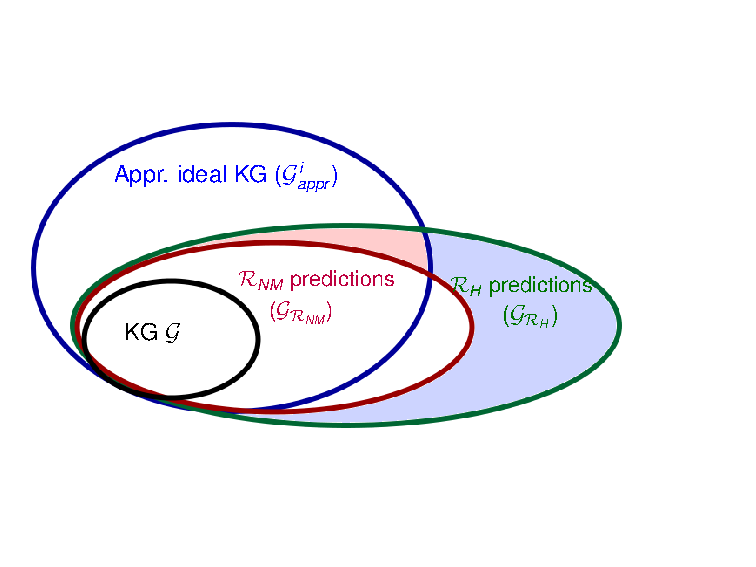
\includegraphics[width=0.5\textwidth]{corr_inc_negl}}\end{picture}}{\begin{picture}(0.5,0.5)\put(93,-83){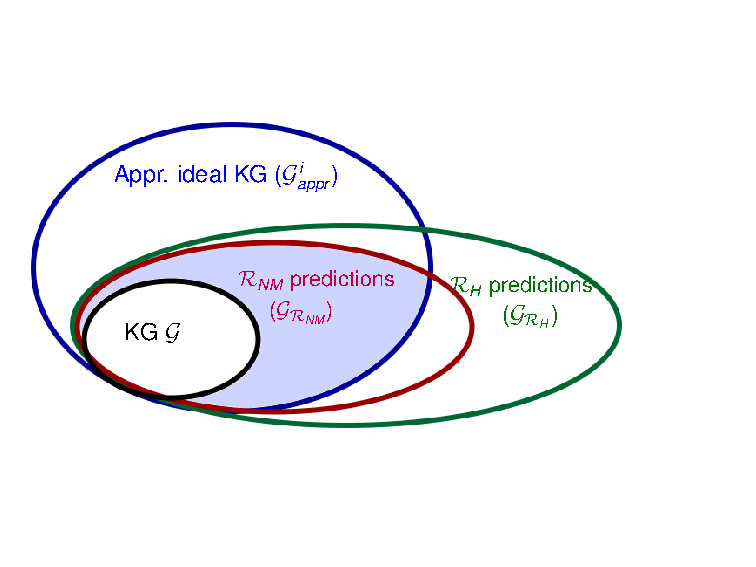
\includegraphics[width=0.5\textwidth]{corr_pred}}\end{picture}}}
% \end{frame}


\begin{frame} \frametitle{Summary}
\textbf{\bl{Contributions:}}
\begin{itemize}
\item Quality-based Horn theory revision framework under OWA
\item Approach for computing and ranking exceptions based on partial materialization
\item Preliminary experiments on a real-world KG
\end{itemize}
\bigskip
\bigskip

\textbf{\bl{Further Work:}}
\begin{itemize}
\item Evidence for and against exceptions from text corpora
\item Partial completeness 
\item Causality of rules, probabilities
\item More complex rules, e.g. with existentials
\end{itemize}
\end{frame}

% \begin{frame}\frametitle{Rule Revision with Web-based Fact-checking}
% \begin{picture}(0.5,0.5)\put(6,-125){\includegraphics[width=0.95\textwidth]{appr}}\end{picture}
% \end{frame}
\appendix

\section{Additional Material}
\begin{frame}[plain,allowframebreaks,allowdisplaybreaks]
  \frametitle{References}
  \bibliographystyle{named}
 \tiny{\bibliography{references}}
\end{frame}


\end{document}

%%% Local Variables:
%%% TeX-PDF-mode: t
%%% TeX-debug-bad-boxes: t
%%% TeX-master: t
%%% TeX-parse-self: t
%%% TeX-auto-save: t
%%% reftex-plug-into-AUCTeX: t
%%% End:
